% ------------------------------------------------------------------------
% -*-TeX-*- -*-Hard-*- Smart Wrapping
% ------------------------------------------------------------------------
%%% Literature Survey --------------------------------------------------

%\addtolength{\topmargin}{-.875in}
%\addtolength{\textheight}{.875in}
%\footskip
%\nonumchapter{Literature Survey}
\chapter{Neurobiological Aspects of  Brain-Computer Interfaces }%Foundations of Brain Computer Interfaces
\label{chap:lit_survey_neuro}
\epigraph{Whenever you remove any fence, always pause long enough to ask yourself, `Why was it put there in the first place?'}{--- \textup{ G.K. Chesterton}}
%-------------------------------------------------------------------------
%\section{Brain computer Interfaces Technology}
%\label{sec:BCI_tech}
%In this section, the Brain Computer Interface (BCI) Technology is discussed. 
%The section is introduced with a presentation of BCI technology, its aim and a quick historical review of major turning points in BCI research \ref{subsec: bci_tech_intro}. 
%The technology of BCI is then presented with each building block of a BCI system described \ref{subsec: bci_tech_components}.
%Different types of BCI as well as elements that mark their differences are presented \ref{subsec:bci_tech_category}.
%After having set the fundamentals of BCIs, the state-of-the-art of the technology is presented \ref{subsec:bci_tech_sate}  
%The section is concluded with a discussion on the limitations in the state-of-the-art and the opportunities thereof.

\section{Introduction}%Quid Est
\label{sec: bci_tech_intro}
%------------------------------
Brain-computer interfaces also called brain-machine interfaces (BMI) are devices that translates measured brain activity into tangible actions, allowing humans and other animals to interact with the physical environment without using their muscular system.
From the 1980s this technology has received growing attention. 
Researchers from various fields including neurology, neuroscience, computer science and electrical engineering have multiplied their effort to move brain-computer interfaces from proof of concept to working prototypes.

Ideas of reading into the human brain were steered up for the first time in 1929 when Hans Berger~\citep{berger_uber_1929} published his work on the recoding of brain electrical activities, \emph{electroencephalograms} (EEG). 
For decades that follow this breakthrough, EEG was used for the diagnosis of neurological diseases and the study of brain functions \citep{wolpaw_brain-computer_2002,daly_brain-computer_2008}. 
A further step was taken when EEG was explored for therapeutic possibilities. People could learn to intentionally control their EEG to limit frequency of seizures in epilepsy, to treat hyperactivity and other disorders~\citep{daly_brain-computer_2008}.

Despite the ability of recording and analysing brain signal, no dive was taken into deciphering brain signals for interaction purposes. 
The idea of reading human thought from brain was contemplated more in fiction than in science.
Relying on brain signals to interact would require detecting human intention from the recorded EEG that was not possible with the early understanding of EEG and its quality. It was impossible to recognise a brain activity induced by a specific intention from the vast electrical activity of neurons. Moreover a detection of intention would require a real-time analysis of EEG which was not foreseeable with the technology at hand. 

The first attempt of using measured brain signals as carriers of information in man-computer communication or for the purpose of controlling external devices came in the 1970s, with the \emph{Brain-Computer Interface project}~\citep{vidal_toward_1973}. 
The project benefited from the advances made in EEG studies providing the evidence that beside the continuous ongoing activity, EEG waves contained time-locked disturbance in response to brief stimuli, and could also be altered by conscious decision~\citep{donchin_discriminant_1969, vidal_toward_1973}.
With very limited computational power at the time, the project constituted a proof of concept that the authors believed would be achievable in the future given considerable advances in neurophysiology, in signal analysis techniques, and in computer science.   

After the \emph{Brain-Computer Interface project}, there were four factors that triggered advances toward brain-computer interface \citep{wolpaw_brain-computer_2002}: the first factor is the advances made in neurophysiology particularly the progress in EEG measurement techniques, the understanding of how EEG was affected by conscious as well as unconscious experience, and better understanding of brain functions. 
The second factor is the development in computing technology and computational power allowing complex and online treatment of EEG.
The third factor is the increasing social need of assisting people with severe motor disabilities especially locked-in people who could not use tradition assistive devices that rely on muscular functions. 
The final factor is the finding that EEG could be used to affect activity-dependent plasticity and contribute to the recovery of motor functions.

Indeed, BCI can be used as a replacement for deficient muscular functions in people with severe motor disabilities who cannot use conventional assistive methods that depend on voluntary muscle control~\citep{wolpaw_brain-computer_2002}. 
The targeted population include people suffering from neuromuscular disorders such as ALS, severe cerebral palsy, brainstem strokes, severe muscular dystrophy or peripheral neuropathy, and other acute disorders causing extensive paralysis~\citep{daly_brain-computer_2008}.  
BCI can also be useful for the rehabilitation of functions that have been lost after accidents that damage the nervous system~\citep{silvoni_brain-computer_2011}.  
 
%\subsection{Brain Computer Interface Components}
%\label{subsec: bci_tech_components}
%----------------------------------
Brain-computer interfaces translate measured brain signals into tangible actions for a specific application. The functionality of such a system requires at least 3 components: a signal acquisition component that measures brain activity, a signal processing component that decipher the measured signal, and an application interface where the deciphered brain activity is used as command.
\begin{figure}[!h]
\centering
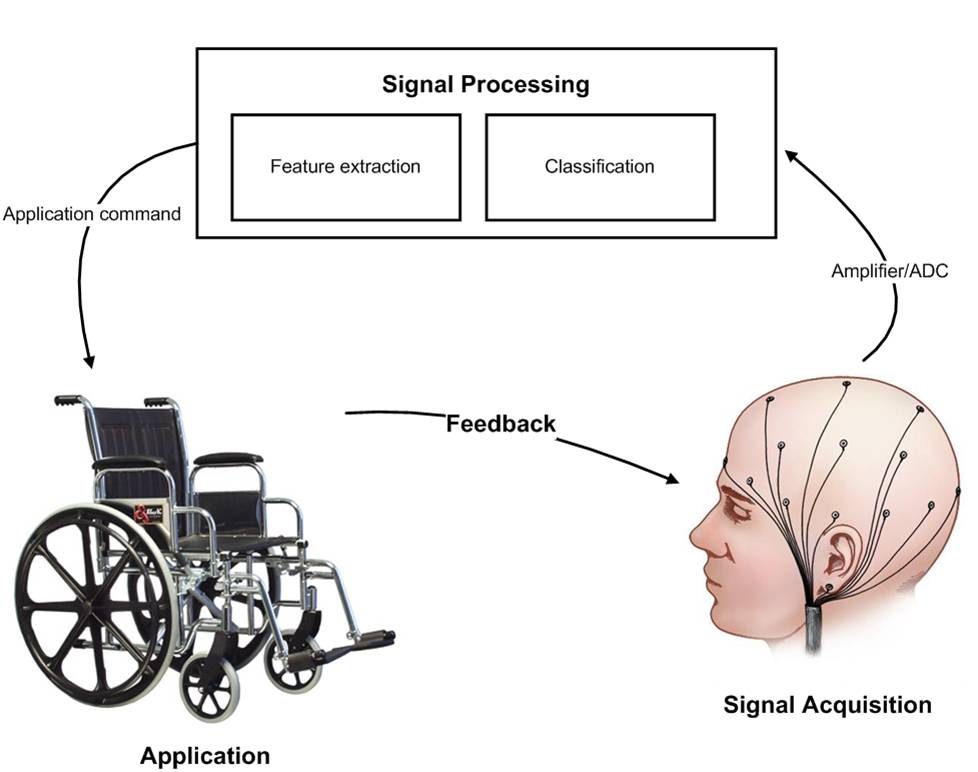
\includegraphics[width=0.5\columnwidth]{Figures/BCI-system}
\caption{A standard BCI system with signal acquisition, signal processing and application components. The system provides feedback to the user.}
\end{figure}

In this chapter, signals used in BCI are presented, along with their measurement techniques, as well as their underlying neurological phenomena.  
%--------------------------------------------------------------------------------------------------------
\section{Signal Acquisition}
\label{sec:signal_aquisition}
To measure brain activity, BCI relies on brain imaging techniques used in neurophysiology. 
The existing methods for brain imaging used in BCI can be grouped in three: electric signals, magnetic signals and hemodynamic signals.
Electric and magnetic signals are two sides of the same coin and can be grouped under the term electromagnetic signals.
%\subsection{Electromagnetic Signals}
\subsection{Local Field Potentials}
\label{neuron_electro}
The brain is made of billions\footnote{The human brain contains about 85 billion neurons~\citep{herculano-houzel_remarkable_2013}.} of interacting neurons constituting a neural network.
A neuron is made of three major parts: a cell body, an axon, and dendrites~\citep{purves_neuroscience_2008}. 
Each neuron can be connected up to thousands other neurons. 
The connection between neurons is made at a junction called \emph{synapse}. 
These junctions are often between an axon of one neuron and dendrites of the next neuron, and are referred to as axon-dendrite synaptic junctions (various other connections exist, e.g. axon-axon, dendrite-dendrite, dendrite-axon). 
The \emph{presynaptic neuron} is passing information to the \emph{postsynaptic neuron}~\citep{herculano-houzel_human_2009,purves_excitatory_2001}.

\begin{figure}[!h]
\centering
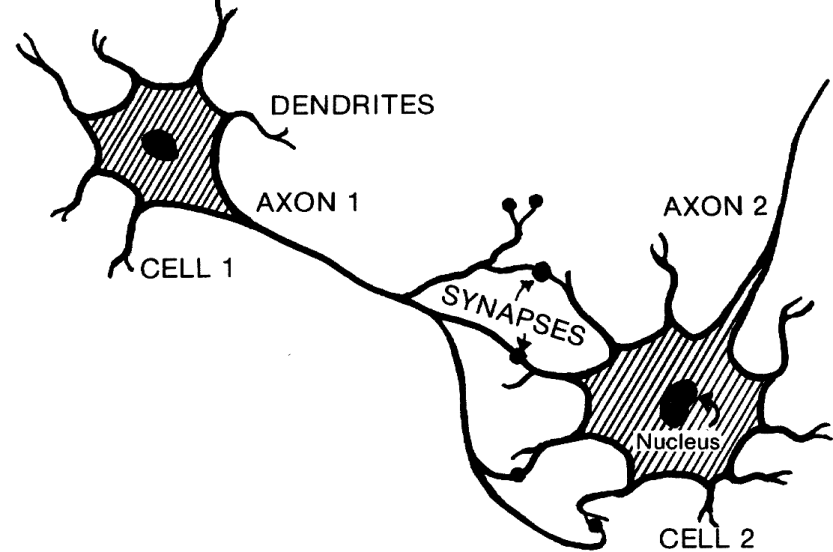
\includegraphics[width=0.5\columnwidth]{Figures/neuron-structure.png}
\caption{Neuron structure: showing main components of a neuron and its axon-dendrite synaptic connection to a neighbouring neuron \citep{purves_excitatory_2001}}
\end{figure}

%Neurons can send either an electrical signal --via \emph{electrical synapses}, or a chemical signal -- via \emph{chemical synapses}.
The information sent between two neurons is mediated by a transient modification of voltage potential called action potential or \emph{spike}.
An activated neuron fires an action potential that is sent through its synapses to its postsynaptic partners. 
The excitatory and inhibitory postsynaptic potentials (EPSPs and IPSPs) cause a flow of charged ions between point at different potentials within and outside the neurons producing an electrical current, called \emph{Local Field Potential} (LFP).
Inside the neuron, positive ions propagate from the subsynaptic area to the rest of the neuron. 
Outside the neuron, the ions that have entered the cell are replaced by an ion flow directed toward the synaptic region along the extracellular space.
%The magnetic effect of the created flow of current generates a magnetic field that propagates orthogonally to the flow of current. 

\begin{figure}[!h]
\centering
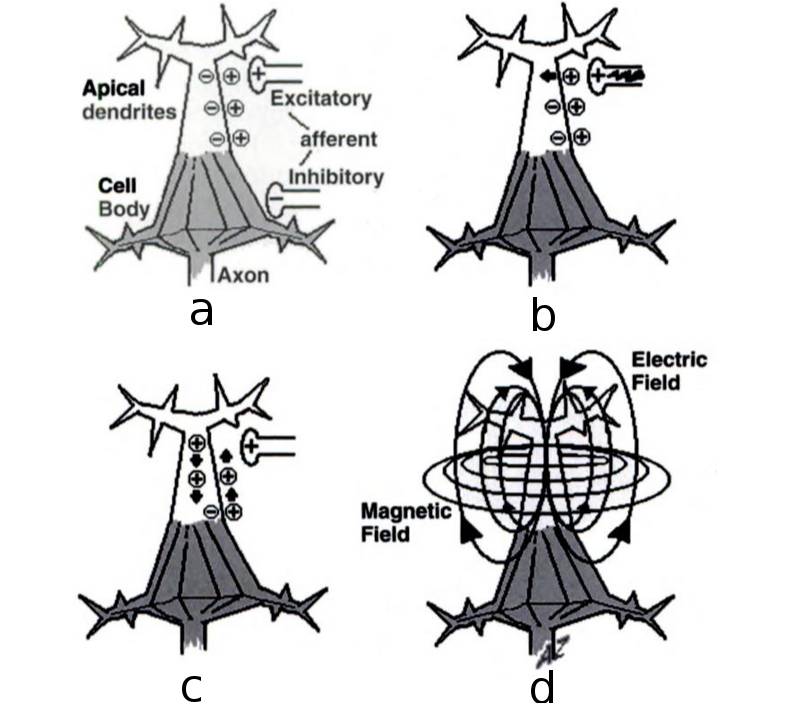
\includegraphics[width=0.5\columnwidth]{Figures/neuron-electromagnetic}
\caption{Electromagnetic activity in pyramidal neuron: (a) EPSPs converge to apical dendrites of the neuron. (b-c) Positive ions enter the neuron and propagate from synapses to the rest of the neuron. (d) the flow of current perpendicular to the apical dendrite is accompanied by a magnetic field that propagates orthogonally. \citep{proverbio_electromagnetic_2003}}
\end{figure}

\subsection{Electrical Signal Acquisition}
\label{elec_acquisition}

There are nowadays various techniques used to measure neuron electrical activities.
They can be measured on the scalp, on the cortical surface, or within the cortex.
\begin{figure}[!h]
\centering
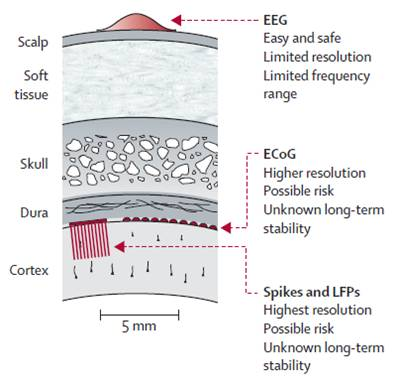
\includegraphics[width=0.5\columnwidth]{Figures/cranial-layers}
\caption{A cut through cortical layers. Electric activities can be measured from different layers. \citep[Reproduced from][]{daly_brain-computer_2008}}
\end{figure} 

\textbf{Electroencephalography} is the measurement of the brain electric activity on the scalp. 
It is the most used measurement technique in brain-computer interfaces, and is at the origin of the expansion of BCI technology. 
Electrodes are spread over the scalp to cover all regions of the cortex. 
%Few electrodes placements have been proposed with the most adopted configuration being the \emph{international 10-20 system}~\citep{niedermeyer_electroencephalography:_2005}.

%\begin{figure}[h!]
%\centering
%\subfigure[]{
%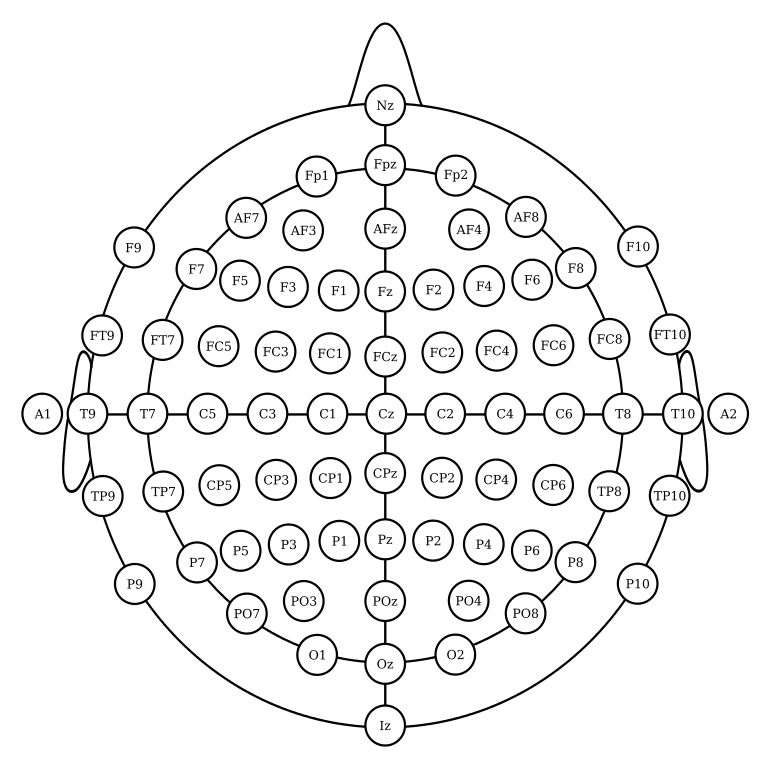
\includegraphics[width=0.5\textwidth]{Figures/eeg-electrodes-10-20}
%\label{fig:eeg-10-20}
%}
%\subfigure[]{
%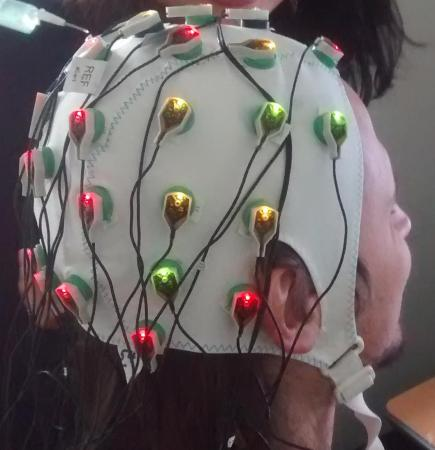
\includegraphics[width=0.45\textwidth]{Figures/eegcap}
%\label{fig:eegcap}
%}
%\caption{EEG measurement: (a) 10/20 system EEG electrodes configuration. The distance between two consecutive
%electrodes is either 10\% or 20\% of the total front-back or right-left distance of the skull. (b): Electrodes cap being fitted on a subject's head for EEG recording.} 
%\label{fig:swel_alpha}
%\end{figure} 

The changes in electrical potentials -- \emph{electroencephalogram} (EEG), recorded at an electrode are the sum of electric field of neurons that are perpendicular to the scalp beneath the electrode. 
The recorded EEG is in the order of microvolts.
EEG is recorded at an acquisition rate that can go as high as 1000 samples per second, providing a good time resolution. However, its spatial resolution is very low. It contains no depth information about the source. 
Moreover due to the dipole-like propagation of the electric potential of the source, the maximum of the distribution does not coincide with the source localisation~\citep{proverbio_electromagnetic_2003}. 
The volume conduction affects the potential field as different biological layers do not have the same electrical properties and are inhomogeneous. 
%Electricity propagate differently in different media. 
The spatial resolution of EEG is affected by this, as the measured electrical field travels through different layers of the skull.
EEG can measure brain electrical activities in spectral bands from 0 to 100 Hz. In BCI, it usually measures activities of up to 40 Hz, \textit{i.e} lower gamma band \citep{schalk_brain-computer_2011}. Activities in the upper gamma band, \textit{i.e.} from 35 Hz to 100 Hz, have been measured mostly in emotion analysis \citep{li_emotion_2009, muller_processing_1999}. 

\textbf{Electrocorticography} measures the same activity as EEG, but the electrodes that measure \emph{electrocorticogram} (ECoG) are placed directly on the exposed  surface of the cortex.  
For this reason it is also referred to as \emph{intracranial electroencephalography} (iEEG).
EcoG were recorded in humans and animals since the late 19$^{th}$ century \citep{caton_electrical_1875}.
Since then, ECoG has been used more in animals due to the fact that the placement of electrodes requires a skull surgery.
%, which is not readily doable in humans.
The study of ECoG in humans is mostly done in epileptic subjects who await surgery. 
ECoG electrodes are temporarily placed to monitor epileptic seizures and locate their focus zone~\citep{ritaccio_proceedings_2012}.
It is only very recently that ECoG has been considered for BCI~\citep{huggins_detection_1999, pfurtscheller_spatiotemporal_2003}. 
The first BCI using ECoG in humans was done by \cite{leuthardt_brain-computer_2004}.
Most BCI research is done on epilepsy patients and should coincide with the time ECoG electrodes are implanted for surgical purposes. This limit the number of ECoG-based BCI. 
There are few rare cases where ECoG electrodes have been implanted exclusively for research purposes~\citep{wang_electrocorticographic_2013, sutter_brain_1992}.

%- Electrode placement
ECoG electrodes are usually in the form of electrodes array on a grid (Figure \ref{fig:ecog}) placed above (epidural) or below (subdural) the dura mater, \textit{i.e.} the tough layer between the skull and the cortex ~\citep{schalk_brain-computer_2011}.
The location of electrodes array is determined by the clinical need in epilepsy patients~\citep{bundy_decoding_2016}. 
For patients who have the ECoG electrodes implanted exclusively for research purposes, a fMRI is done prior to the placement to determine the cortical zone of interest for the BCI task~\citep{wang_electrocorticographic_2013}.   
%- Image
%\begin{figure}[!h]
%\centering
%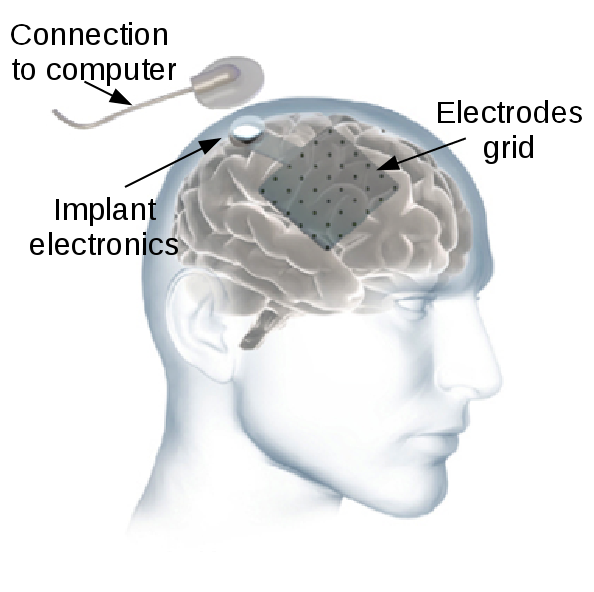
\includegraphics[width=0.3\columnwidth]{Figures/ecog-electrodes-legend}
%\caption{ECoG Electrodes. Courtesy of Ripple, Inc}
%\end{figure}

%- Acquisition frequency->time resolution - Spatial resolution - Bandwidth
ECoG is recorded at rates higher than 1 kHz, giving it a very high time resolution. 
The fact that the electrodes are placed directly on the surface of the cortex gives ECoG higher spatial resolution (\textit{i.e.} 1.25 mm for subdural recording and 1.4 mm for epidural recording~\citep{schalk_brain-computer_2011}), wider frequency bandwidth (0 to 500 Hz), and higher amplitude (\textit{i.e.} 50 to 100 $\mu V$) than EEG~\citep{schalk_brain-computer_2011, leuthardt_brain-computer_2004, spuler_decoding_2014}.
With a wider bandwidth, ECoG can capture neural electrical activity in the $\gamma$-band -- which ranges from 30 Hz up, with higher precision than EEG. 
ECoG BCI research has shown that activity in the $\gamma$-band provide deeper information about movement and movement imagery such as direction and velocity both 2-dimensional and 3-dimensional \citep{bundy_decoding_2016, leuthardt_brain-computer_2004}.

\begin{figure}[h!]
\centering
\subfigure[]{
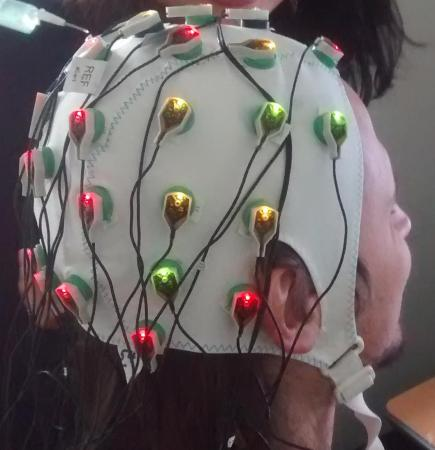
\includegraphics[width=0.3\textwidth]{Figures/eegcap}
\label{fig:eegcap}
}
\subfigure[]{
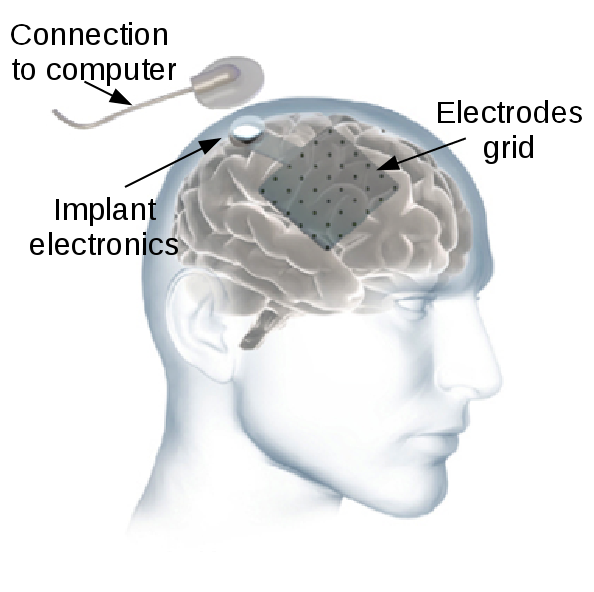
\includegraphics[width=0.3\textwidth]{Figures/ecog-electrodes-legend}
\label{fig:ecog}
}
\subfigure[]{
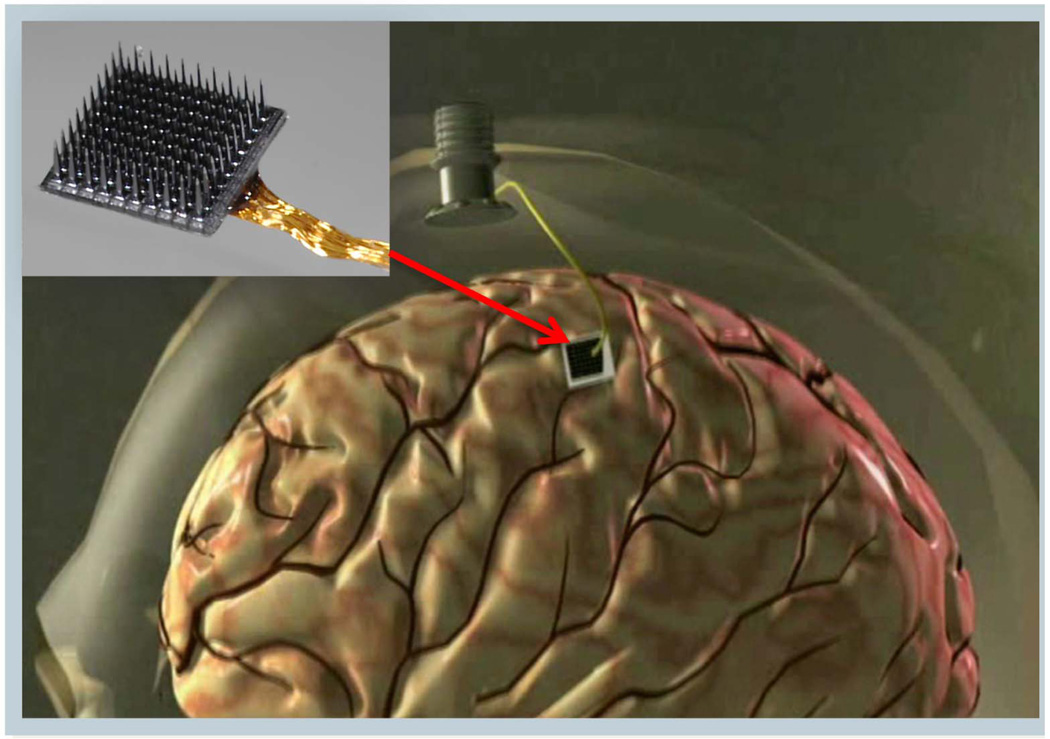
\includegraphics[width=0.3\textwidth]{Figures/intracranial-electrodes}
\label{fig:intracranial}
}
\caption{electric signals electrodes: (a) EEG electrodes cap being fitted on a subject's head for recording. (b) ECoG Electrodes. Courtesy of Ripple, Inc. (c) A silicon-based cortical MEA (inset); implanted for intracortical neural recording via a percutaneous connection to a skull mounted pedestal connector \citep{homer_implants_2013}.} 
\label{fig:electrodes-electric}
\end{figure} 

    
\textbf{Spikes} and \textbf{Local Field Potentials} are intracortical measures of neural activities. 
The purpose is to measure the activity of a single neuron via its spikes, or the sum of activities of a small population of neurons local to a region -- the local field potentials.
Recording of neuronal spikes done approximately 50 years ago has shown that movement intent modulates spike timing from neurons of the motor cortex. 
%\begin{figure}[!h]
%\centering
%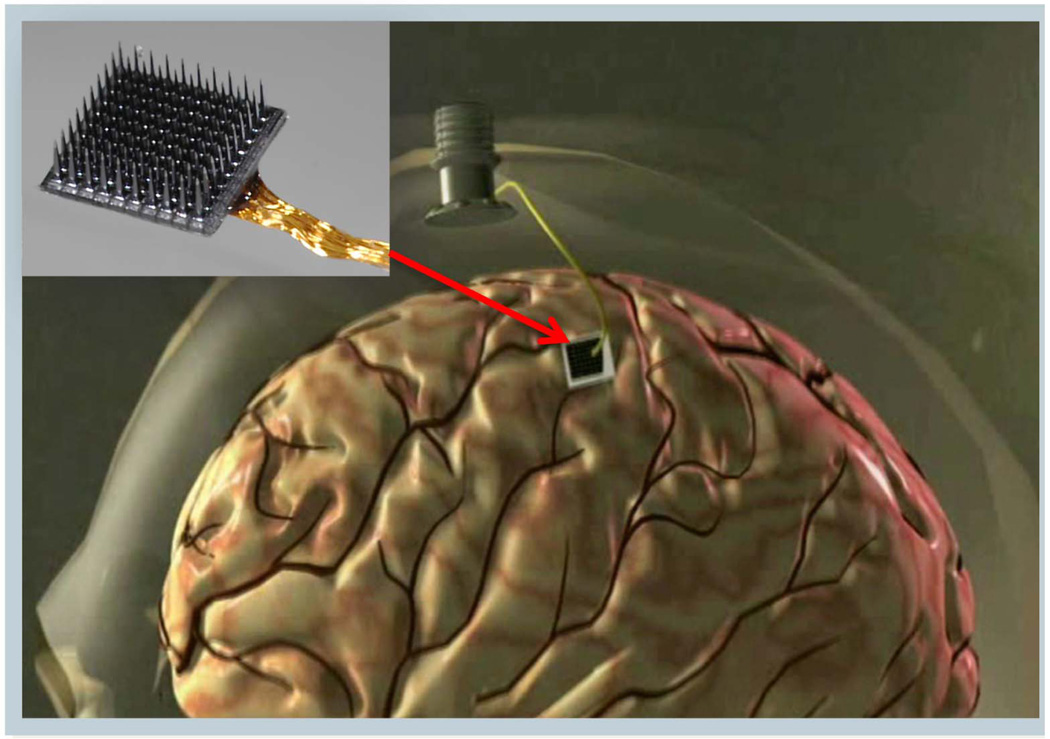
\includegraphics[width=0.5\columnwidth]{Figures/intracranial-electrodes}
%\caption{A silicon-based cortical MEA (inset); implanted for intracortical neural recording via a percutaneous connection to a skull mounted pedestal connector \citep{homer_implants_2013}.}
%\end{figure}

The first clinical application using intracortical recording -- also called stereoelectroencephalography,  was achieved in 1998~\citep{kennedy_restoration_1998}.
The electrodes are placed in the motor cortex. 
A fMRI or MRI is performed before the implant to locate the precise location.
From the year 2000, substantial research has been done on these recording techniques, mostly on non-human primates~\citep{serruya_brain-machine_2002, taylor_direct_2002, musallam_cognitive_2004, santhanam_high-performance_2006, golub_motor_2014}. 
It has shown that it is possible to control devices such as prosthetics and achieve complex tasks such as 3D control, and reaching and grasping action with prosthetic devices by using motor cortex spiking pattern~\citep{homer_implants_2013}.
%Studies done on monkeys have paved the way to intracortical BCI for humans. 
In humans, intracortical BCI has been studied on patients with spinal cord injuries~\citep{hochberg_neuronal_2006,hochberg_reach_2012}, amyotrophic lateral sclerosis~\citep{kennedy_restoration_1998}, brainstem stroke~\citep{kennedy_direct_2000}, and mitochondrial myopathy~\citep{kennedy_computer_2004}.
By recording activities of individual neurons, recorded signals are not affected by activities happening in different brain regions. With electrodes implanted in different regions of the cortex, intracortical BCI could take parallel commands and offer many degrees of freedom. 
      
\subsection{Magnetic Signal Acquisition}
\label{magnet_aquisition}
Electric and magnetic signals are two side of the same coin. 
They are both created by the same synaptic exchange between neurons~\ref{neuron_electro}.
The magnetic effect of electric currents in neurons generates a magnetic field that propagates orthogonally to the flow of current~\citep{gazzaniga_cognitive_2013, proverbio_electromagnetic_2003}. 

\textbf{Magnetoencephalography} (MEG) is the measure of neurons magnetic field on the scalp. 
It is a neuroimaging technique used in neuroscience and clinical applications. 
It is very related to EEG as both are measured on the scalp. 
Both magnetic and electric fields propagate through different cranial layers before being measured on the scalp.
Nonetheless MEG has an advantage over EEG; the magnetic field is not as influenced by the medium as is the electrical field. 
A drawback in measuring the magnetic activity of brain is that it is 
8 orders of magnitude bellow 
%100 millionth the size of 
the earth's magnetic field (in the order of $10^{-15}$ Tesla). 
Due to this, it cannot be measured in ``open air".
Electromagnetic isolation chambers are needed, making the MEG acquisition equipment bulky and expensive. 
MEG sensors are usually made of a magnetometer and two orthogonal planar gradiometers. 
Ranging from 64 to more than 300, MEG sensors are immersed in liquid helium and attached on a concave bottom of a container, where they typically lie at a distance of  3 - 4 cm from the cortex. 
The weak extracranial magnetic fields are amplified and transformed into a voltage \citep{paetau_magnetoencephalography_2002}.



\begin{figure}[h!]
\centering
\subfigure[]{
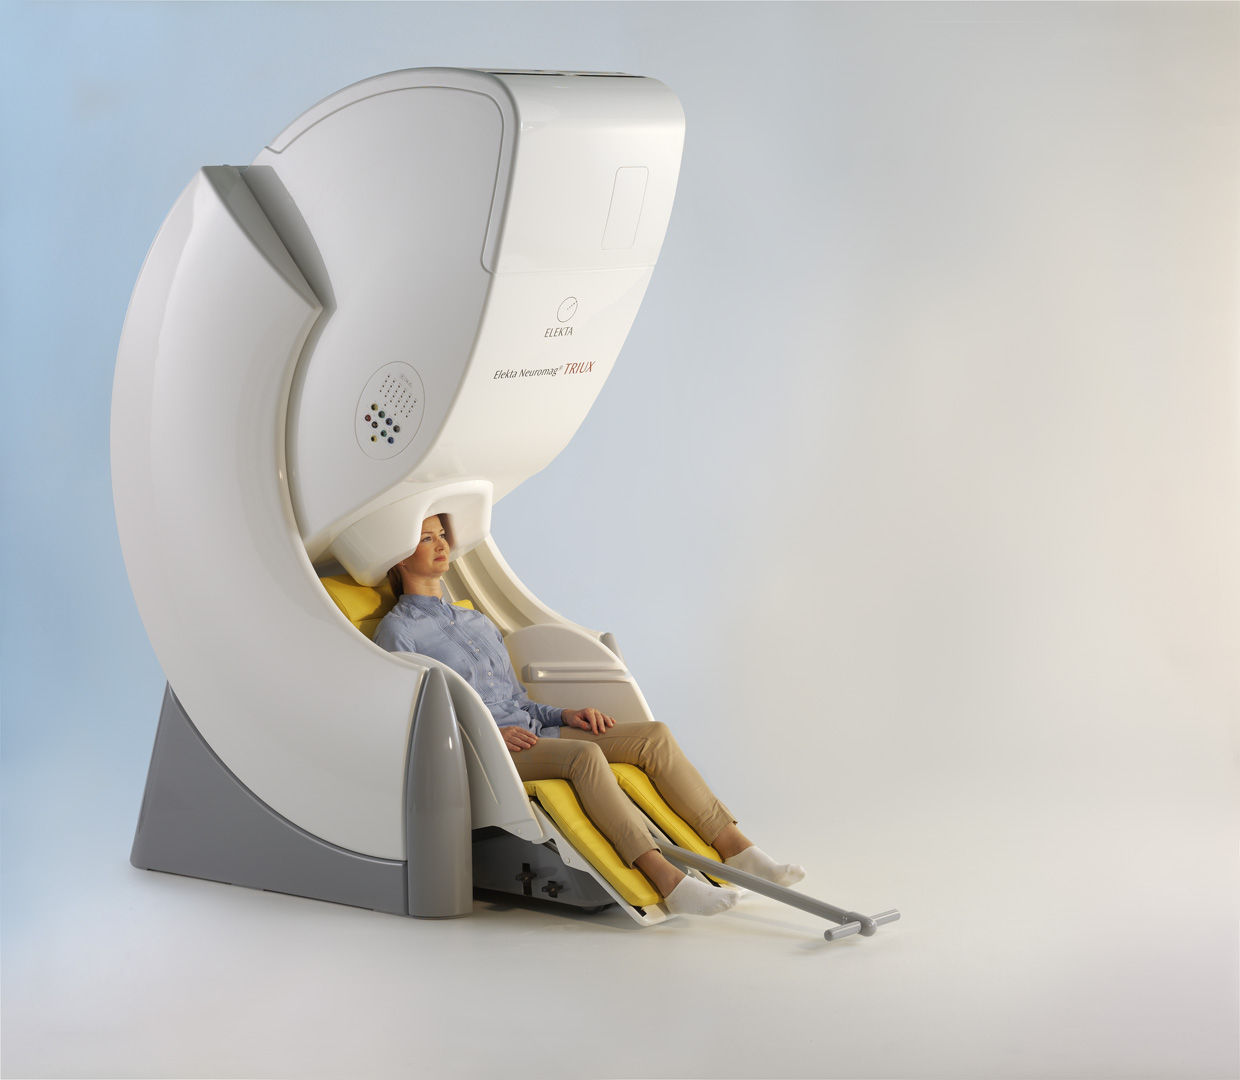
\includegraphics[width=0.45\textwidth]{Figures/MEG_scanner_elekta}
\label{fig:meg-sys-chamber}
}
\subfigure[]{
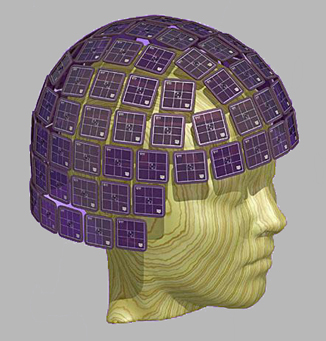
\includegraphics[width=0.45\textwidth]{Figures/MEG_sensors}
\label{fig:meg-sys-sensors}
}
\caption{Elekta MEG acquisition system. (a) A MEG shield chamber for electromagnetic isolation  (b) MEG sensors configuration. Each sensor location is equipped with three sensors: a magnetometer  that measures normal field component, and two orthogonal planar gradiometers that measure gradient components~\citep{team_elekta_2016}.}
\label{fig:meg-system}
\end{figure} 

MEG has similar temporal resolution to EEG, but has a higher spatial, and can better capture modulations in brain signals, thus improving control and information transfer rates in BCI. 
EEG and MEG can also be co-recorded in BCI tasks and used in to improve BCI performances \citep{mellinger_meg-based_2007, henson_parametric_2011, foldes_meg-based_2015}.

\subsection{Hemodynamic Techniques}
\label{optical_sig}

While EEG, ECoG, LFP, spikes, and MEG measure the direct electromagnetic activities of neurons, there are other neuroimaging techniques that measure the metabolic effect of neurons electrical activities.
In fact there is a relationship, \textit{i.e.} \emph{neurovascular coupling}, between neuronal activity and subsequent regional blood volume and flow.
This coupling is explained by the fact that firing neurons involved in a neurological task requires more energy and oxygen, resulting in an increase of blood flow and oxygenation. 
The active neurons in the region do not use the totality of the provided oxygen. 
This results in a change in the ratio between oxygenated (oxyHb) and deoxygenated (deoxyHb) hemoglobin. 
This metabolic response to neuron activities is called the \emph{hemodynamic response} and can be measured using different techniques such as Magnetic Resonance Imaging (MRI), Functional Magnetic Resonance Imaging (fMRI), Positron Emission Tomography (PET), Near Infrared Spectroscopy (NIRS), and Functional Near Infrared Spectroscopy (fNIRS).
fMRI, NIRS, and fNIRS have a possibility of real time recording required for brain-computer interfaces.

\textbf{fMRI} or Blood-oxygen-level-dependent (BOLD) fMRI uses magnetic resonance to measure the concentration of oxyHb and deoxyHb making use of the difference in their magnetic properties \citep{matthews_functional_2004, gosseries_[functional_2008, huettel_functional_2004, sitaram_fmri_2008}.
fMRI consist of multiple scans of MRI to capture brain activity. 
A transmitter coil covering the head is needed to generate a magnetic field responsible for the resonance and relaxation in oxyHb and deocyHb. 
fMRI have high spatial resolution (i.e few millimetres) and low temporal resolution (\textit{i.e.} few seconds) compared to electromagnetic brain signals.
fMRI-BCI capitalises on the ability of fMRI to locate brain activity to the millimetre, to characterise different spatial distribution of brain functions as BCI commands \citep{sitaram_fmri_2007, yoo_braincomputer_2004}. 
Though fMRI-BCI can achieve high classification accuracy, they are held back by the low temporal resolution that limit the speed of MRI scans and the information transfer rate of the interface.
Furthermore, the size and setup of fMRI acquisition equipment limit the mobility of users.

\textbf{NIRS} and \textbf{fNIRS} are recent hemodynamic techniques introduced in the late 1980s. 
They measure the intensity of light propagated through brain tissues. Since the concentrations of oxyHb and deoxyHb in brain tissues are indicators of neural activity, f/NIRS use the relationship between transmitted light and the concentration of the medium (i.e chromophores such as oxyHb and deoxyHb) to calculate these concentrations by shining near-infrared light on the head and measuring the intensity of the exiting light as shown in Figure \ref{fig:nirs}.

\begin{figure}[h!]
\centering
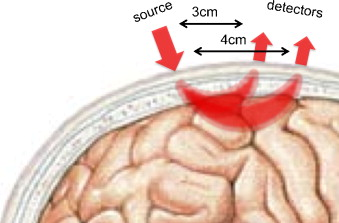
\includegraphics[width=0.45\textwidth]{Figures/nirs}
\caption{Trajectory of near-infrared light in the human brain. \citep[Reproduced from][]{gervain_near-infrared_2011}.}
\label{fig:nirs}
\end{figure} 

f/NIRS has a good spatial resolution (few millimetres), better compared to electromagnetic signals measured on the scalp (\textit{i.e.} EEG and MEG), but lower than fMRI.
The acquisition equipment is lighter, easy to use, and enhances mobility of the subject. 
NIRS is tolerant to movement whereas other signals' recording techniques either does not allow user movement (e.g. fMRI, MEG) or the signal quality is distorted by movement (e.g. EEG).
As with fMRI-BCI, f/NIRS-BCI also relies on the ability to separate brain function based on their spatial distribution. 
%Though it spatial is lower compared to fMRI, f/NIRS-BCIs are easier to use. 
Although the spatial resolution of f/NIRS is lower than the resolution of fMRI, f/NIRS-BCIs are easier to use than fMRI-BCIs.
They have good classification accuracy, but are still slower than BCI that use electromagnetic signals. 
The BCI tasks are also limited to brain functions that can be measured close to the scalp. 
In fact f/NIRS cannot measure deep brain activity, because of light penetration which is limited to 15 mm and 5~mm into the cortex, for infants and adults respectively. 

%that has the merit of enhancing the mobility of the subject. While in EE 

%*The fact that it is also an indirect measurment of neuronal activity give it a low temporal resolution similar to fMRI.(sampling freq <= 10) but is faster than fMRI (0.5Hz)

\subsection{Discussion}
\label{subsec:signal_acq_discussion}

Several neuroimaging techniques have the potential of being used in BCI. 
Each has characteristics that can be used to successfully classify brain functions.
One requirement that all should meet to be considered as an input signal in BCI applications is the ability of near real time recording/scanning. 
%They also have limitations that will limit their efficacy in BCI. 
%A trade-off should be decided on to choose an optimal signal for BCI.

Neuroimaging techniques such as fMRI and MEG limit the mobility of the user and limit  brain-computer interface to few applications. 
Moreover fMRI is not real time.
Despite their good spatial resolution and temporal resolution (for MEG), they are not adapted for daily life interaction. 
f/NIRS is a good trade-off between user mobility and spatial resolution of the acquired signal. 
However, the fact that, as fMRI, it relies on hemodynamic response implies a low temporal resolution that might not be enough to capture transient brain responses to stimuli used in BCI, and exposes it to physiological noise such as cardiac cycle and respiratory effect that alter blood oxygenation more than other measurement techniques. 
In terms of user mobility and ability to capture fast brain response, electrical signals (EEG, ECoG and intracortical signals) remain so far the best options.
It is proven that intracortical BCIs offer high interaction performances by decoding complex brain activities. 
However the risk and uncertainties surrounding the intracortical implantation of electrodes are still an issue for its recognition by the public. It is judged to be too invasive.
The intracranial version of EEG -- ECoG, alleviates many problems of EEG-based BCI, namely its vulnerability to noise (\textit{i.e.} ocular, muscular and environmental). 
Although it is less invasive compared to intracortical measurement, ECoG still requires surgery for electrodes placement. 

Despite its relatively low spatial resolution and vulnerability to noise, EEG remains the sole technique that offers fast tracking of neural activities, affordable and light recording equipment allowing BCI users' mobility, safety and ease of use.
It is vastly adopted as the input signal for BCI. 
However, some researchers believe that the future of BCI lies in invasive techniques. 
They argue that non-invasive techniques can only represent a limited number of brain responses -- thus limited degrees of freedom, and that EEG weaknesses are hardly overcome. 
Another argument is that, for the same neurological phenomenon, non-invasive BCI requires longer training periods for the users  to learn to produce a particular brain response voluntarily, and despite the training non-invasive BCI still have high error rates. %~\citep{birbaumer_brain-computer-interface_2006}. 
A further argument is that although non-invasive medically, EEG measurement technique can also be seen as invasive in terms of human machine interaction: the gel, the tight electrode cap, the restriction to blink eyes during recording, etc. might be seen as invasive.
These arguments have not stopped the EEG-based BCI community from pushing the limits. 
Wolpaw and McFarland disapproved the argument against non-invasive BCI by showing that with a comprehensive user training and good learning algorithms, EEG-based BCI could provide multidimensional point-to-point movement control that falls within the range of invasive BCI performances~\citep{wolpaw_control_2004}.
Research on improving EEG-based BCI performance has increased all the more, with better tools for the processing of EEG signals \citep{gramfort_mne_2014}, and encouraging results \citep{mattout_improving_2013, kalunga_online_2016}.  

In conclusion, while other neuroimaging might be adequate for some BCI applications (e.g. neurofeedback), EEG constitutes a reasonable choice for signal input in BCIs for assistive purposes (e.g. communication and mobility). 
EEG-based BCIs are well tolerated with their limitations by patients with the need to communicate without their muscular systems~\citep{kubler_severity_2005, grubler_psychosocial_2014}. 
With effort from different fields involved in BCI research, it is possible to reach better performance and tend toward those reported with invasive BCIs.  

  
%\subsubsection{Signal Processing}
%- Explain the steps that are taken and examples of each
%\subsubsection{Application interface} %Mention Feedback
%- Name applications of BCI and examples, and how feedback is provided
%
%Brain computer interfaces decipher brain signal characteristics related to subject intention or reaction to a stimulus into tengible action. 

%\subsection{Brain Computer Interface Categorisation}
%\label{subsec:bci_tech_category}
%\subsection{Neurological Phenomena}
%\label{subsec:bci_tech_neuro_phenomena}
%
%\subsection{Brain Computer Interface Performance Evaluation}
%\label{subsec:bci_tech_performance_evaluation}
%
%\subsection{Brain Computer Interface state-of-the art} %Mention successful examples of BCI and present their performance
%\label{subsec:bci_tech_sate}
\section{Neurological Phenomena}
\label{sec:lit_survey_neuro_phenomena}

In deciphering brain signals, brain-computer interfaces identify a specific feature -- a \emph{neurological phenomenon}, from the signal that is associated with a given user's intention. 
Neurological phenomena are variations in the brain signals associated with a cognitive activity (\textit{i.e.} cognitive conscious information processing),  or in response to a physical stimulus.
Neurological phenomena induced by cognitive activities are said to be \emph{endogenous}, while those triggered by external physical stimulus are said to be \emph{exogenous}.
Respectively, BCIs that rely on exogenous neurological phenomena are classified as exogenous or dependent BCIs as they dependent on an external stimulus, and their counterparts that rely on endogenous phenomena are classified as endogenous or independent BCIs as  no external stimulus is needed.
BCI research has mainly focused on the following phenomena: Event Related Desynchronisation (ERD) and Event Related Synchronisation (ERS), Event Related Potential (ERP), and visually Evoked Potential (VEP). 
There are discussed in the details in the next lines.
%####################################################################################################################################
\subsection{Event-Related Synchronisation-based BCI}
\label{subsec:ERD/S-BCI}

\subsubsection{Event-Related Desynchronisation and Synchronisation}

%Several kinds of events -- sensory or motor -- induce events-related
%potentials in the brain signals. 
%
%Manifested as deflections in the brain
%signal's voltage, event-related potentials are believed to be a result of a reorganisation of the phases or changes in specific frequency bands in the ongoing brain signals \cite{pfurtscheller1999ERDreview}. 
Event related (de)synchronisation are either a decrease --\emph{event-related desynchronisation} (ERD), or an increase -- \emph{event-related synchronisation} (ERS), of power in a given frequency band during a cognitive activity\citep{pfurtscheller_graphical_1977, pfurtscheller_event-related_1977, pfurtscheller_event-related_1994}; they are endogenous phenomena. 
%The former is called event-related desynchronisation or ERD and the latter event-related synchronisation or ERS \cite{Pfurtscheller1977Graph} \cite{Pfurtscheller1992} \cite{Pfurtscheller1977Event}.

\par \cite{pfurtscheller_event-related_1999} interpret ERD as an electrophysiological correlate of activated cortical areas involved in processing of sensory or cognitive information or production of motor behaviour. 
ERD/ERS is mainly observed in the 
$\alpha$ rhythm, the $\mu$ rhythm also referred to as the upper $\alpha$ rhythm, the $\beta$ rhythm and the $\gamma$ rhythm.
The $\alpha$ rhythm ranges from 8 to 12~Hz, the $\mu$ between 10 and 12~Hz, the $\beta$ rhythm between 12~ and 30~Hz, 
and the $\gamma$ rhythm between 30 and 60~Hz.
The low frequencies of oscillations in the brain signal are caused by synchronous neural activities that involve a large number of neurons. 
Hence slow oscillations are measurable in a large area of the brain. 
On the other side, assemblies of only small numbers of neurons in synchrony  oscillate at high frequencies \citep{singer_synchronization_1993}.  
The amplitudes of oscillations being proportional to the number of synchronous neurons, low frequencies have higher amplitude and high frequencies smaller ones. Therefore ERD/ERS in $\alpha$-rhythm are more visible than in any other
frequency bands.% (ie. high amplitude and wide topographical distribution). This is illustrated in Figure~\ref{fig:alphawave}.

%\begin{figure*}[!ht]
%    \centering
%    \includegraphics[width=4.0in]{Figures/alphawave.pdf}
%    \caption{\footnotesize{EEG recorded on 8 channels in the occipital region. The signal
%    is band filtered from 8 to 60Hz. The amplitude (y-axis) is in $\mu$-volts
%    and the time (x-axis) in seconds. The subject is relaxed with closed eyes.
%    A synchronisation in the alpha wave of approximately 10Hz is visible on
%    all channels with high amplitude.}}
%    \label{fig:alphawave}
%\end{figure*}

Though easily measurable, lower $\alpha$ wave ERDs cannot be used to discriminate between tasks due to their wide topographical distribution. 
Moreover they might be obtained in response to any task. % \cite{pfurtscheller1999ERDreview}. 
$\mu$ rhythm ERDs, however, are topographically restricted to some brain areas and happen only in response to specific activities. $\mu$-rhythm ERD provoked by a given task will be observed mainly in the brain cortex in charge of the task. 
This specificity to tasks offers a possibility of discrimination amongst them~ \citep{pfurtscheller_event-related_1999}.
%This offers a possibility for discrimination between tasks. 

\subsubsection{Motor Imagery BCI Systems}

The cognitive tasks used in current ERD/ERS-based BCI systems include motor imagery \citep{pfurtscheller_motor_2001}, mental tasks, e.g. sitting idle, doing a multiplication, composing a song \citep{kumar_design_2010}, composing letters, counting, rotating objects \citep{faradji_brain-computer_2009}), or a combination of mental tasks and motor imagery tasks \citep{penny_eeg-based_2000, ozmen_discrimination_2011}.% \cite{Penny2000EEG-based,Ozmen2011Discrim}. 

A user performs a cognitive task while his brain signals are being recorded, for further processing and classification.
The majority of studies conducted in ERD/ERS-based BCI are carried out on synchronous systems. 
Figure~\ref{fig:ERDSparadigm} illustrates a synchronous ERD/ERS-based BCI paradigm. 
The mental task is performed from the cue onset for a specific period of time. The trial starts with a beep. The user looks at the screen -- where a fixation cross is displayed -- waiting for the cue that will indicate the mental task to be performed. 
\begin{figure*}[!ht]
    \centering
    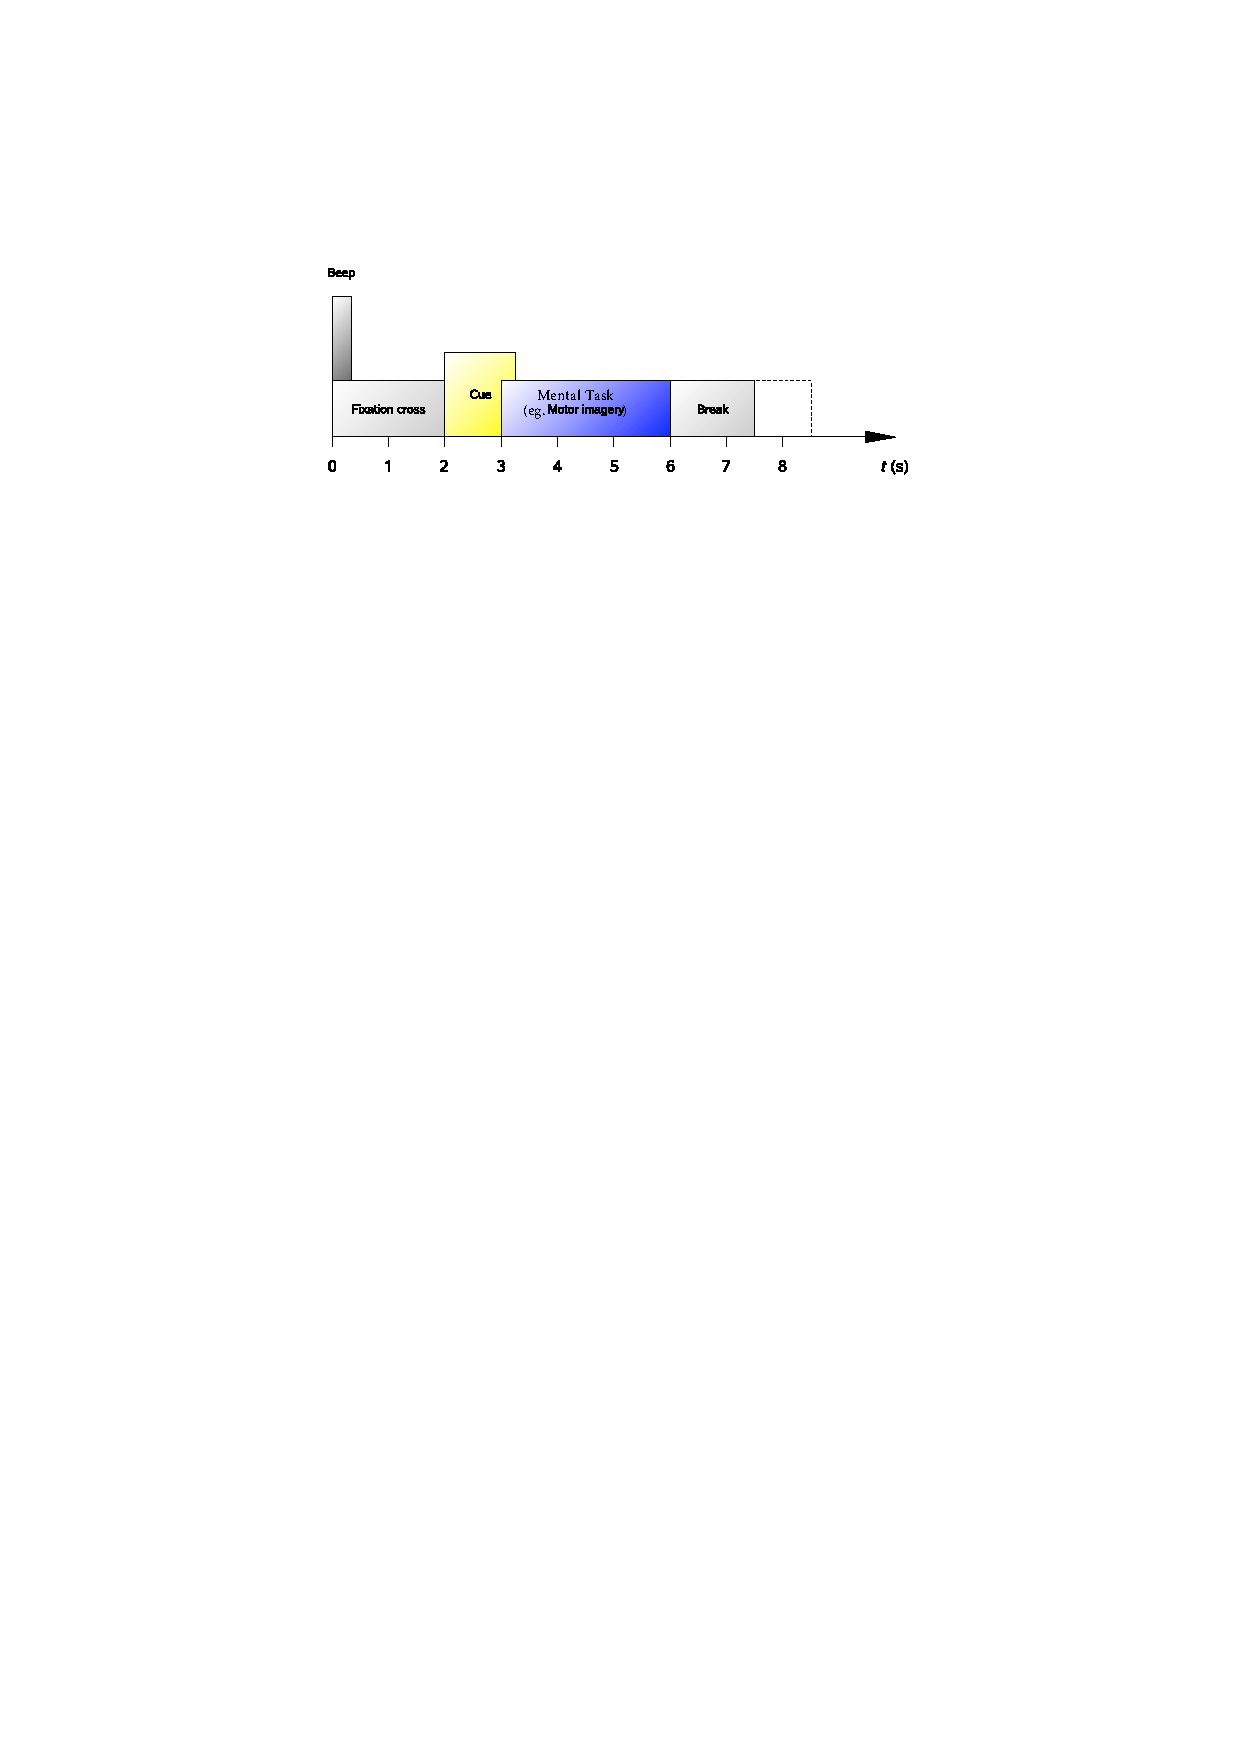
\includegraphics[width=0.5\columnwidth]{Figures/ERDS-paradigm.pdf}
    \caption{\footnotesize{Standard ERD/ERS-based BCI system paradigm. The
    break before the next trial should last at least a second to allow the changes in the
    ongoing EEG/MEG to recover. }}
    \label{fig:ERDSparadigm}
\end{figure*}
\par

Motor imagery provides the most intuitive and affordable cognitive task for the large population of users and has therefore dominated BCI research. It also has a record of best classification accuracy. 
The tasks that induces the most separable features in the EEG are the imagery of right-hand movement, the imagery of left-hand movement, the imagery of foot movement and the imagery of tongue movement~\citep{ang_filter_2012}. 
When a person is at rest (\textit{i.e.} not involved any motor activity), there is a high  activity in the 8-12 Hz band (\textit{i.e.} $\mu$ rhythm) and the 18-26 Hz band (\textit{i.e.} $\beta$ rhythm) in the motor cortex. This activity is also known as \emph{sensory motor rhythm} (SMR).
It has been shown that for right hand movement there is a decrease, ERD, of SMR in the left hemisphere of
the sensory-motor cortex, and the ERD occurs prior to the actual movement, during the preparation phase preceding the movement \citep{pfurtscheller_event-related_1999}. 
It has also been established that motor imagery (mental imagination of movements) activates similar brain areas (functions) to those activated during the preparation phase of actual movement \citep{jeannerod_mental_1995, roland_supplementary_1980}.
In general, voluntary hand movement results in bilateral ERD in the hand area and ERS in the foot area (see homunculus in~\ref{fig:homunculus}); while a simple mental imagination of the same movement results  in the contralateral  $\beta$ ERD and ipsilateral $\beta$ ERS, both in the hand area \citep{pfurtscheller_existence_1997, pfurtscheller_event-related_1994, toro_c._and_deuschl_g_and_thatcher_r_and_sato_s._and_kufta_c_and_hallett_m._event-related_1994}.
The fact that in mental imagination of one-sided hand movements the ERD remains mostly limited to the contralateral hemisphere is of key value in the classification of motor imagery-based BCI. 
%Left and right hand imagery can be differentiated on the grounds of their asymmetrical electrocortical responses.
%Only these tasks provide a possibility of topographical discrimination between their respective elicited
%ERD/ERS in the $\mu$ and $\beta$ rhythm. 
Several studies \citep{lotte_review_2007} have focused on the imagery of right hand and left hand movement -- since these two tasks present the most discriminative characteristics because of their asymmetrical electrocortical responses -- to build a 2-class BCI and have the best classification accuracy achieved in ERD/ERS-based BCI \citep{zhang_bci_2012}. 
It is to be mentioned that ERD elicited by motor imagery of different parts of an upper limb cannot be discriminated \citep{pfurtscheller_event-related_1999}. 
For instance, the imagery of left wrist movement and any left finger movement will activate the same brain region (contralateral ERD and ipsilateral ERS in the hand region) as the one activated during the imagery of the left hand. 
For lower limbs, imagination of either foot movement results in a $\mu$ or $\beta$ ERD in the foot area between both hemispheres such that it becomes impossible to discriminate between imagery of the left foot and of the right foot \citep{pfurtscheller_event-related_1999}. It is expected that the imagery of foot movement activates the foot area and the imagery of the tongue, the tongue area. 
%However it is generally observed that these tasks result in ERD across unexpected brain areas, making the classification task more difficult. 
However it is generally observed that the area activated by these two tasks are mixed up and not easily interpretable. 

BCI systems must therefore use some complex algorithms to extract the most discriminative features and achieve a multiclass discrimination, e.g. 4-class: right hand, left hand, feet, and tongue~\citep{dornhege_boosting_2004, brunner_spatial_2007}.

\begin{figure*}[!ht]
    \centering
    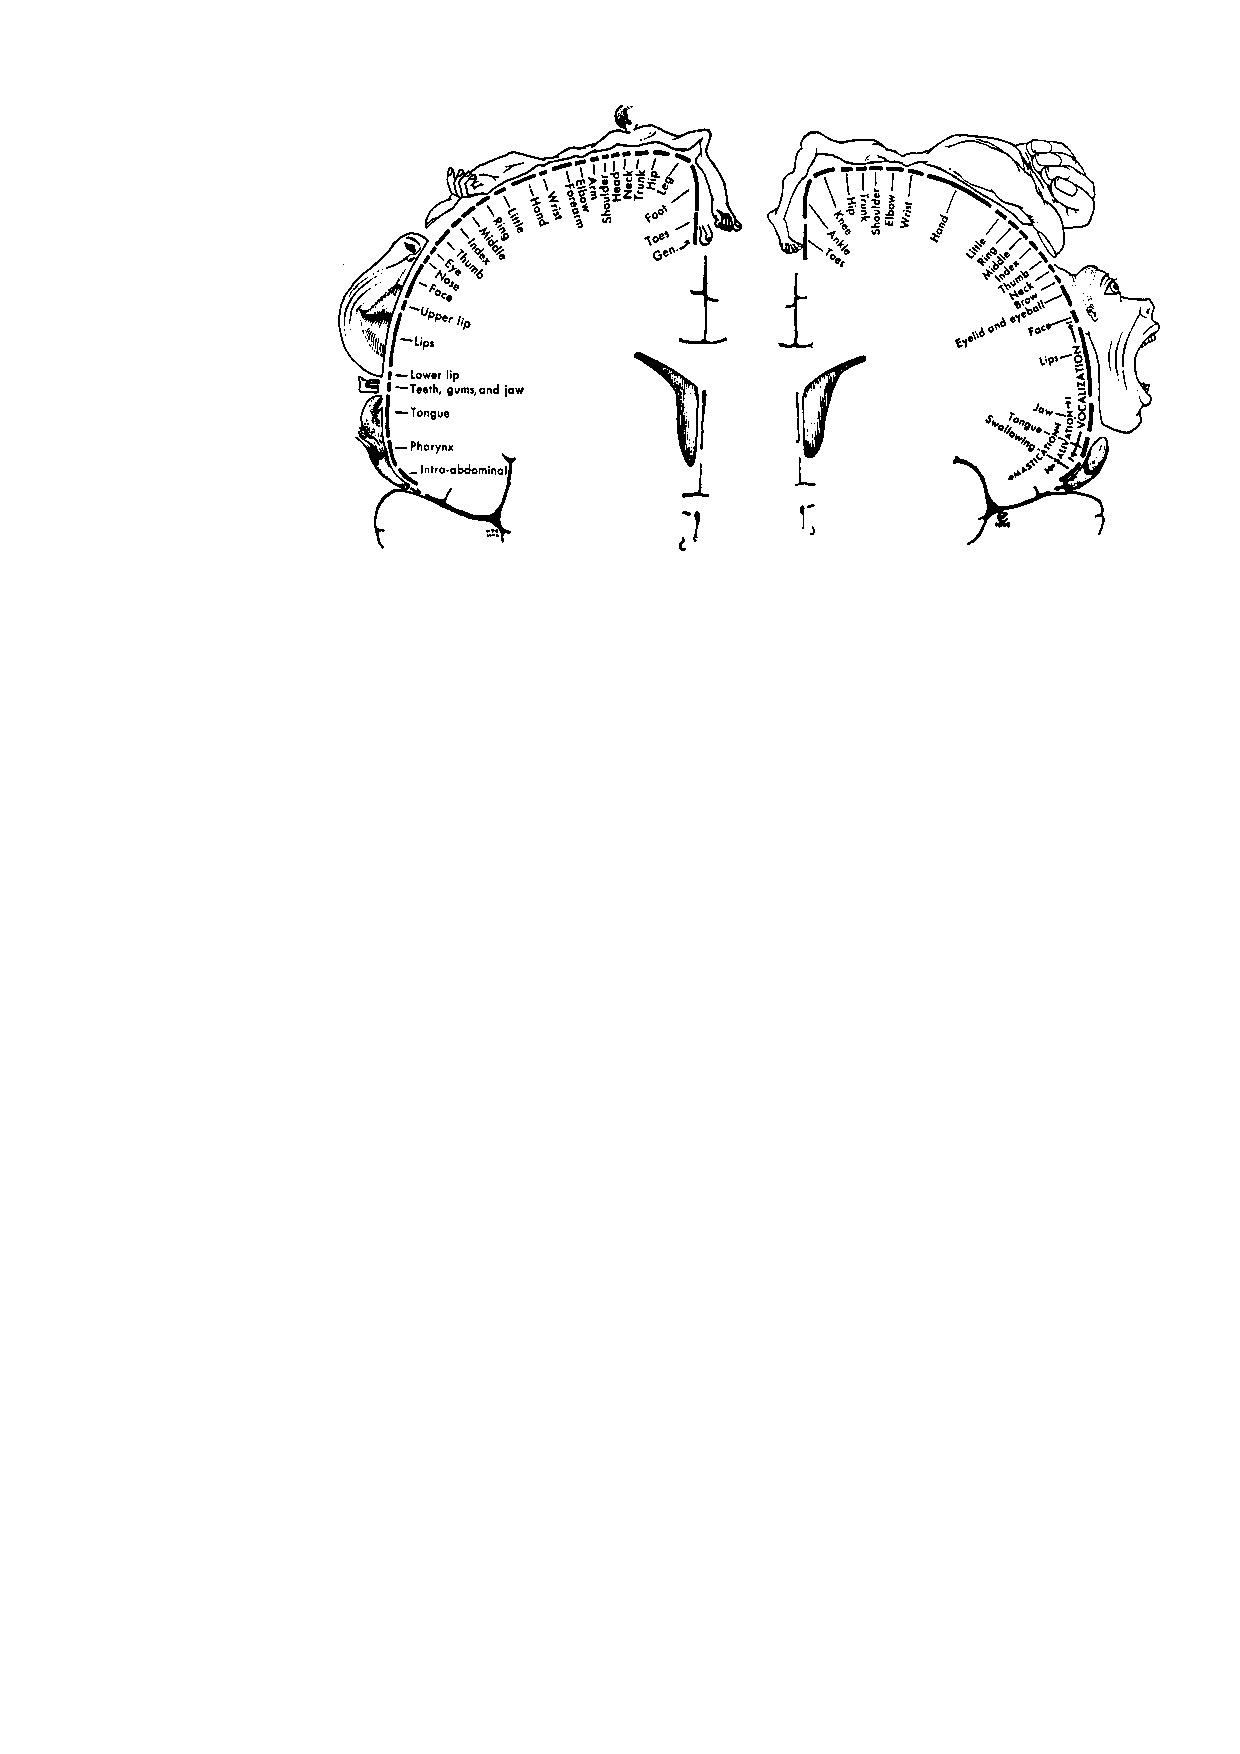
\includegraphics[width=4.0in]{Figures/homunculus.pdf}
    \caption{Sensory homunculus on the left and Motor homunculus on the right.
    The cortical homunculus initially developed by Dr. Wilder Penfield
    shows a disproportionate human body laid on the cortex from the prefrontal
    cortex(top) to the cerebellum (bottom). The size of a given body part
    of the homunculus is descriptive of the amount of cerebral tissue or cortex
    devoted to the specific body region which is proportional to how richly
    innervated that region is.
    This image is taken from \citep{schoot_penfields_1993} }
    \label{fig:homunculus}
\end{figure*}


%\note{something on other mental tasks? see references at the begining of section}
%The majority of studies conducted in ERD/ERS based BCI are carried out on
%synchronous systems. Figure~\ref{fig:ERDSparadigm} illustrates a synchronous
%ERD/ERS based BCI paradigm. The mental task is performed from the cue onset
%for a specific period of time. The trial starts with a beep. The user looks
%at the screen -- where a fixation cross is displayed -- waiting for the cue
%that will indicate the mental task to be performed. New approaches are being
%developed for the implementation of asynchronous ERD/ERS based BCI
%\cite{Satti2009,Lotte2008,Galan2008} where the BCI system continuously
%classifies the ongoing brain activities, not only into a specific class
%corresponding to the performed mental task, and differentiates between IC and
%NC states.
%
%\begin{figure*}[!ht]
%    \centering
%    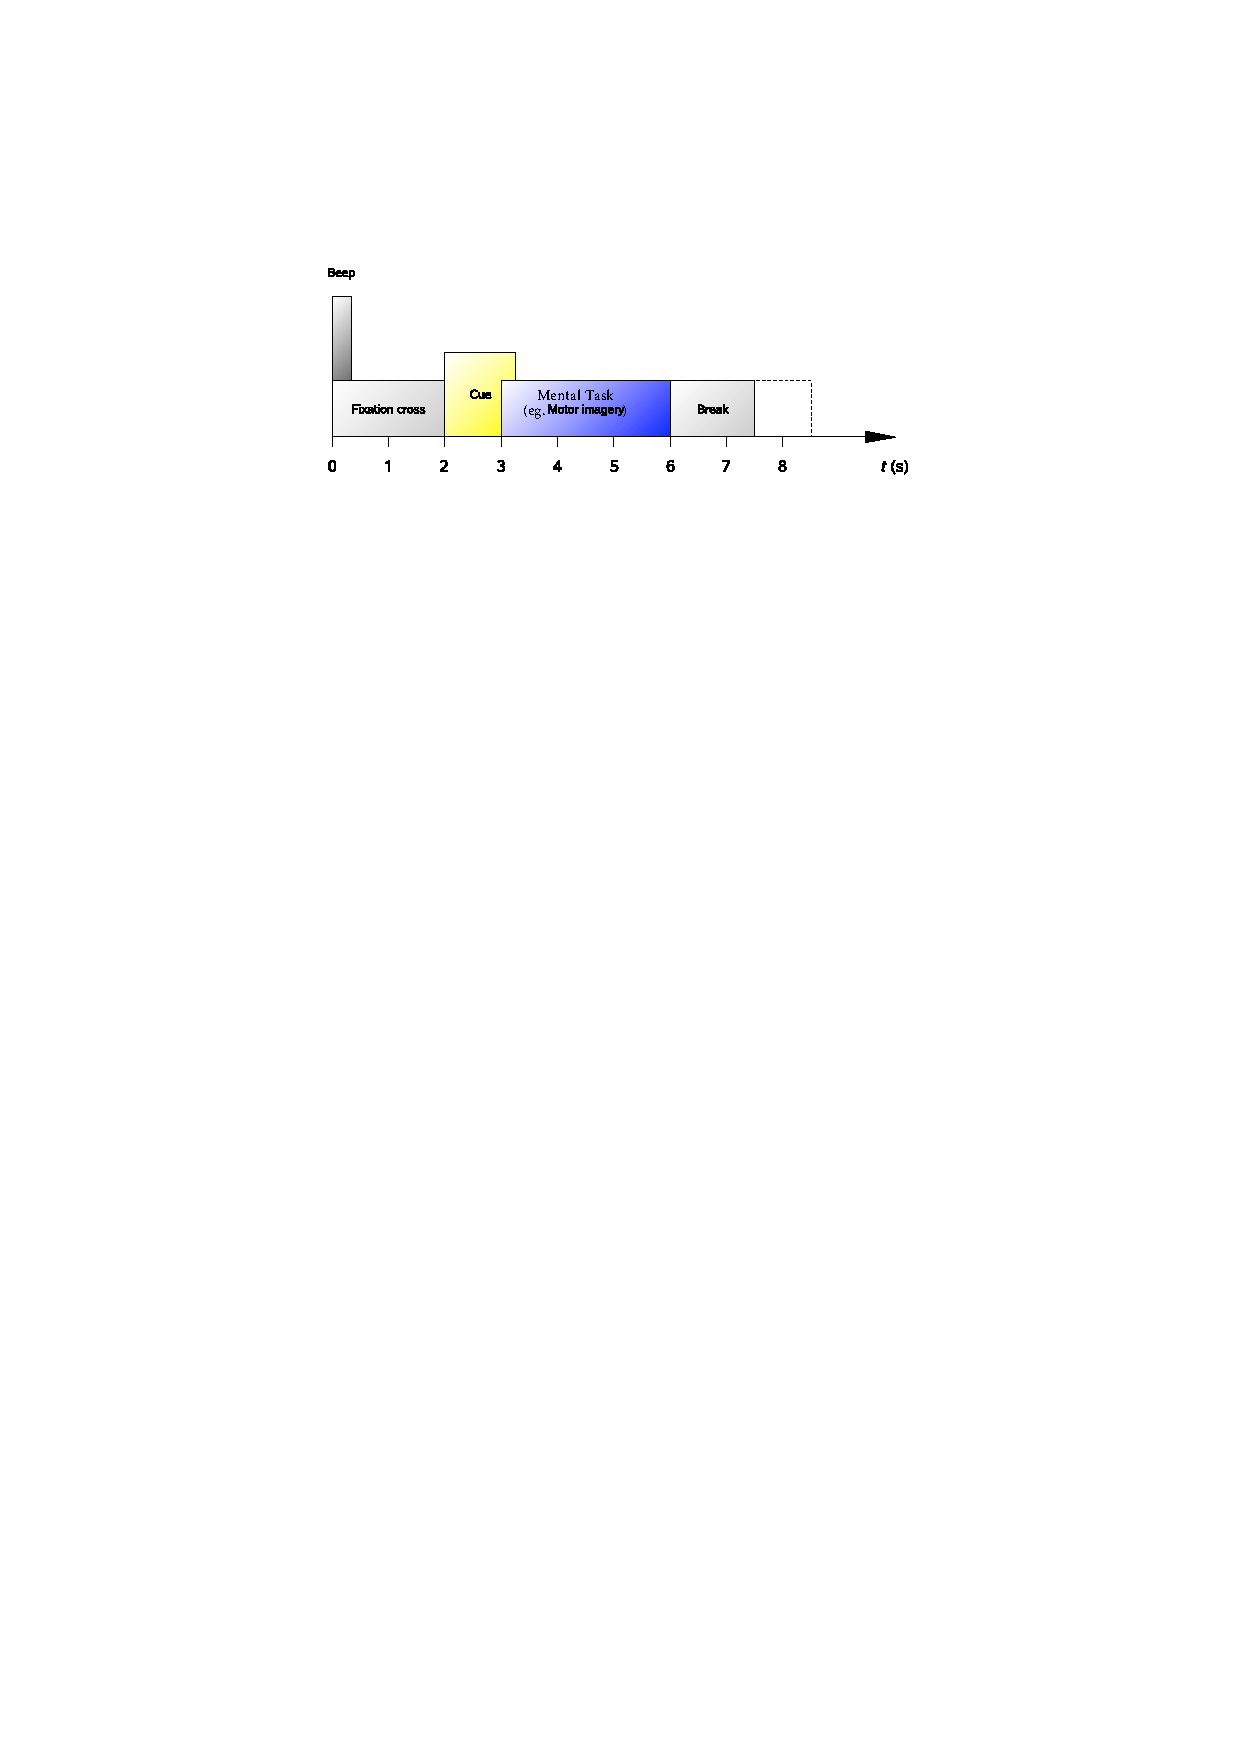
\includegraphics[width=4.0in]{Figures/ERDS-paradigm.pdf}
%    \caption{\footnotesize{Standard ERD/ERS based BCI system paradigm.The
%    break before the next trial should last at least a second to allow the changes in the
%    ongoing EEG/MEG to recover. }}
%    \label{fig:ERDSparadigm}
%\end{figure*}
%\par

\subsubsection{Challenges in ERD/ERS-based BCI systems}

BCIs relying on ERD/ERS face a number of challenges: 
First is the low signal-to-noise ratio. ERD/ERS phenomena are submerged in a much larger brain activity.
It is thus difficult to distinguish a synchronisation or desynchronisation in a single trial. 
%The method used for the quantification of ERD/ERS relies on some kind of averaging methods over many
%trials. BCI systems -- in the signal processing component -- have to enhance
%ERD/ERS and extract the most separable features from a single trial. 
%\par

Secondly, classification into classes representing different intentions is based on the topographical distribution (activated brain regions) and the ERD/ERS frequency range. 
However, as noted, EEG has poor topographical resolution and relatively narrow bandwidth. 
ERD/ERS in ECoG and other signals with better spatial resolution are reported to possess better signal characteristics for classification \citep{wilson_ecog_2006, schalk_brain-computer_2011, power_automatic_2012, naseer_classification_2013, wang_electrocorticographic_2013}. 
Spatial filters are needed to alleviate the poor topographical resolution. 
The impact of spatial filtering on can be seen in \citep{hill_classifying_2006}.

Moreover, ERD and ERS areas are not always the same in different subjects due to physiological differences between them. 
The (de)synchronised frequency band is also not the same amongst subjects. 
Besides, the time where (de)synchronisation happens with reference to a cue is not the same either. 
This forces the BCI systems to identify the relevant brain area (e.g. spatial filter), the frequency band, and the time interval of significant (de)synchronisation \citep{yang_time_2014}. 
The last task becomes even more complex in asynchronous BCI systems where there is no cue, therefore no reference (baseline). 
The term ERD implies that a baseline measured some seconds before the event represents a larger synchronisation \citep{pfurtscheller_event-related_1999}.

A major problem in ERD/ERS-based BCI systems is the user training required. 
Users need to learn how to perform the cognitive tasks such that they can modulate their brain signals in a way that is detectable by the BCI system. 
Even after training, some users still cannot produce signals that are classifiable by the system. This phenomenon is known as \emph{BCI illiteracy} and affects an estimate of 15 to 20\% of BCI users \citep{allison_could_2010}. 
Though the problem of BCI is not exclusive to ERD/ERS BCI, it is more prominent here \citep{hammer_psychological_2012}.
There are many attempts to explain the causes of BCI illiteracy and possible ways of alleviating the problem \citep{allison_could_2010,hammer_psychological_2012,jeunet_why_2016}.

%In terms of information transfer rate, assuming a perfect classification
%accuracy and a negligible processing time, ERD/ERS based BCI systems are
%limited by the minimal length of a trial. As shown in~\ref{fig:ERDSparadigm}, the trial and the inter-trial must be long enough to
%allow event-related changes in ongoing EEG to develop and to recover.

%####################################################################################################################################

\subsection{Event-Related Potential}
\label{subsec:erp}

Event Related Potentials (ERP) are time-locked deflections in the EEG voltage (or electrical activity of a population of neurons) in response to a sensory stimulus. 
A commonly accepted hypothesis is that they are the result of a reorganisation of the phases or changes in specific frequency bands in the ongoing brain signals \citep{pfurtscheller_event-related_1999}.
Having a very small amplitude compared to the ongoing brain activity, they are extracted through an averaging of aligned signal segments of repeated trials. 
After averaging, only the time-locked phenomena will remain, and all unrelated EEG will cancel out. 

The resulting ERP consists of several positive and negative deflections called components of the ERP.
They are designated with a `N' (for negative components) or `P' (for positive components) followed by a number indicating the time when they happened after the stimulus.
Each component reflects a neural process involved in the response to the stimulus.
The first components are usually sensory processes (\textit{i.e.} P120 is the first positive component observed in response to a visual stimulus).
%, N170 reflect the neural processing of face perception). 
They are then followed by more complex processes such as decision, recognition, and emotion related processes. 
N250 reflects the neural processing of a person's own face, P300 reflects the processing of an odd event, N450 marks a processing of conflict, Error Related Potential is negative component observed after an error committed in a selection task \citep{luck_introduction_2014}. 

Only the P300 \citep{polich_updating_2007, donchin_surprise!_1981} and the error related potential (ErrP) \citep{miltner_event-related_1997} components have been explored in BCI applications. 
ERPs are mere responses to sensory stimuli. 
A user would not have a voluntary control of the ERPs and cannot use them as input to a BCI.
The \emph{oddball paradigm} has allowed a ``pseudo'' voluntary control of P300 components, hence its usability in brain-computer interfaces \citep{ritter_averaged_1969}. 
On the other hand, the ErrP has been used in BCI not as a control input, rather as a feedback channel. 
It allows the detection of errors (from the human and the machine) in human-machine interactions \citep{margaux_objective_2012}.   

\subsubsection{P300}
\label{subsubsec:p300}

P300 is a positive deflection in the ERP, typically 300 ms after the perception of an odd event that creates a surprise effect for the subject \citep{donchin_surprise!_1981}.
%The amplitude of the P300 is correlated with the improbability of the discriminated event.
\begin{figure*}[!ht]
    \centering
    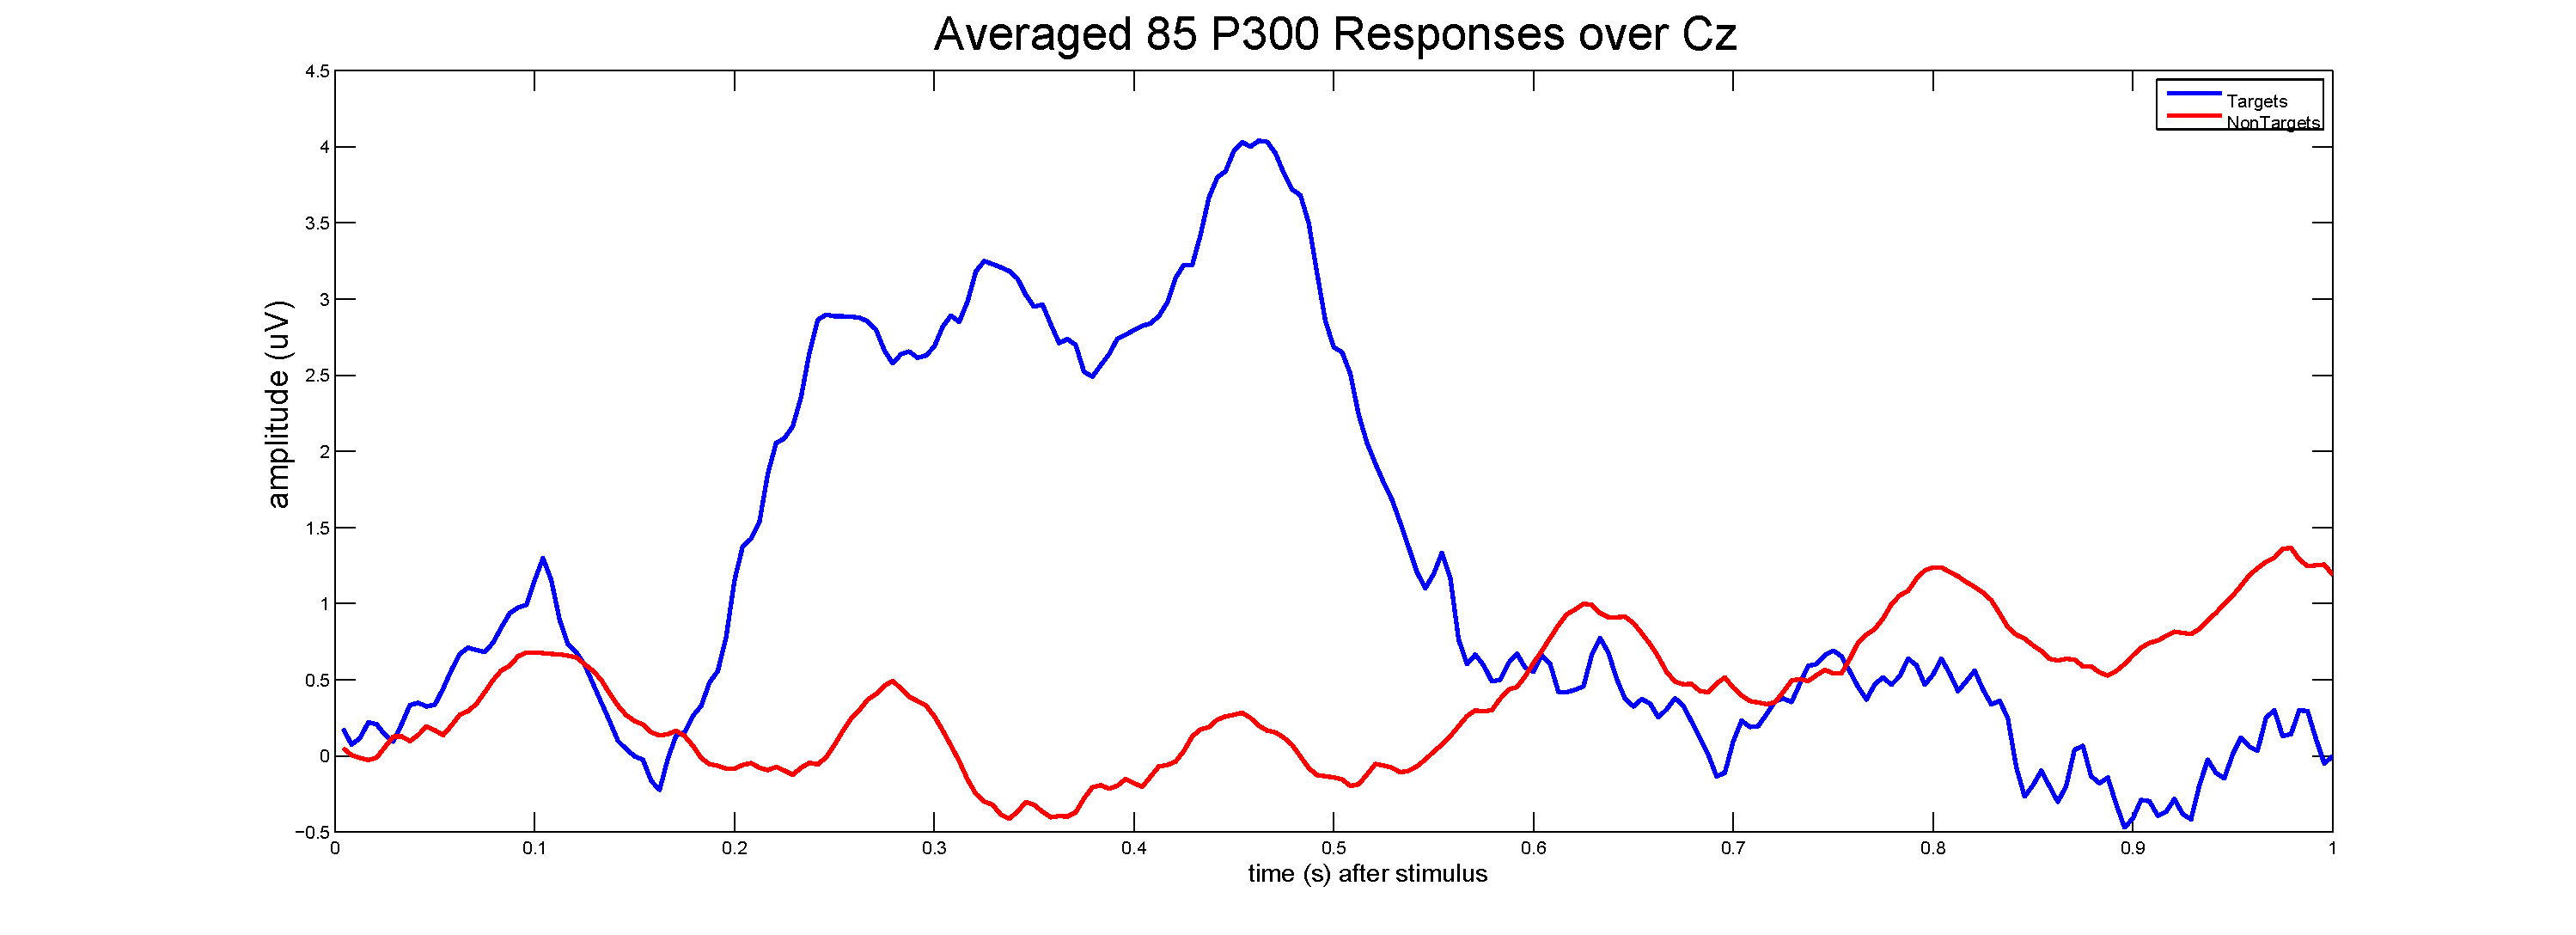
\includegraphics[width=0.5\columnwidth]{Figures/Averaged-85-P300-Responses-over-Cz.pdf}
    \caption{\footnotesize{2550 P300 trials have been averaged to obtain the enhanced P300 (blue line).
    The enhanced P300 is compared to 12750 trials not containing the P300.
    The data used are subject A's recorded signals from the BCI competition III data set II.
    A visual oddball paradigm as described in \citep{donchin_mental_2000} is used to elicit the P300.}}
    \label{fig:85_P300}
\end{figure*}
\par

Contrary to the intuition that P300 might be an exogenous phenomenon, Sutton et al. established that it was endogenous. 
The subject must have perceived the event, analysed it and established its oddity for a P300 to be elicited.
It is related to the psychological reaction of the subject to the stimulus rather than to the physical characteristics of this stimulus \citep{sutton_evoked-potential_1965, sutton_information_1967}.
P300 amplitude is proportional to the temporal probability of the stimulus (e.g. sequential probability) which can roughly be defined as 
($ 1/{\text{total number of stimuli}} $).
It is also, to a lesser extent, related to the stimulus probability: ($\text{stimulus time}/{\text{total trial time}}$) \citep{fitzgerald_temporal_1967}.
\par
P300 has a latency that varies with the difficulty of discriminating the improbable stimulus from the standard ones. 
%For example, while trying to identify, in a series of words, words that are synonymous to ``maverick'', the subject will need some time to process and decide if the word is indeed a synonym, resulting in a longer latency. 
The 300 ms latency is typical in young adults. Older subjects and those with decreased cognitive analogies have smaller P300 with a longer latency. 
Subjects with a greater ability to solve simple problems will generally have shorter latency.
Within the adult population, the latency of P300 increases with age. 
%Polich's review suggests a linear regression of 1.3 milliseconds of latency per year, with a standard error of 31 milliseconds \cite{Polich1991P300inEv}. 
%\par
%The P300 wave is maximally recorded from the midline centroparietal regions. 
%The latency of P300 waves varies from one electrode location to the next, being earlier at more frontal locations. 
Three positive waves overlap during the P300 latency: the P3a near 250 ms, the P3b near 350 ms, and a positive slow wave. 
%The P3a is more frontal than the P3b, while the slow wave is more parietal \cite{Picton1992TheP300}. 
%Depending on the nature of the visual stimulus, the P300 might be larger in the left hemisphere, or larger in the right hemisphere, or just symmetrical \cite{Stapleton1987Endogenous}. 
%When a stimulus was totally unexpected (completely different from the standard stimuli and a new occurrence), the P300 is maximal in the frontal regions \cite{Courchesne1975StimulusNov}.

\subsubsection{P300-based BCI systems}
\label{subsubsec:p300-bci}

In BCI, the \emph{oddball} paradigm is used in a scenario where the subject has a ``pseudo'' voluntary control of P300 generation \citep{ritter_averaged_1969}.  
In this paradigm the subject is presented with a sequence of events that can be classified into two categories, this is the traditional two-stimulus oddball. 
A three-stimulus variation of the oddball paradigm can also be used \citep{polich_updating_2007}. 
In the traditional two-stimulus oddball, events in one of the two categories are rarely presented, thus eliciting a P300. 
%The less probable the eliciting event, the larger the P300 \cite{Donchin2000TheMental}.
\par
Auditory and visual stimuli are used to elicit the P300 with only a few studies focusing on auditory stimuli \citep{elshout_review_2009}. 
Subjects in the complete locked-in state lose all voluntary control and cannot use visual stimuli. 
For such subjects, auditory P300-based BCI could be of great importance. 
Different sounds are played (e.g. notes, words) and for a given task the subject is asked to focus on a particular sound. 
When that sound is played a P300 is elicited around 300 ms later. 
%The BCI system can thus detect the user's intention. Auditory P300s have shorter latency. They typically occur 140 ms earlier than the visual P300. 
Despite the opportunity they represent for people in a complete locked-in state, auditory P300-based BCI have low information transfer rate and have been explored by only a few studies \citep{sellers_p300_2006, elshout_review_2009, kathner_portable_2013, kaufmann_face_2013}.

\par
The most popular application of P300-based BCI systems is the P300 speller \citep{farwell_talking_1988}. 
The subject is presented with a screen, containing a metric of characters. %containing 36 characters arranged in a $6 \times 6$ matrix. 
Rows and columns of the matrix are flashed one after the other in a randomised order. 
The selected character is at the intersection of the row and column which, when flashed, were followed by a P300.
The flashes are repeated several times to enhance the detection of P300 through averaging.
%In another words, when a P300 is generated, the system checks the row or column that was flashed 300 ms earlier. This is repeated a number of time so that both the column and the row of the targeted character are flashed more than once.  
It was pioneered by Farwell and Donchin when for the first time they used the oddball paradigm and the flashing matrix to spell words conveyed to a voice synthesiser. They achieved a communication rate of 12 bits or 2.3 characters per minute \citep{farwell_talking_1988}.
Since then, several improvements have been made. 

\begin{figure*}[!ht]
    \centering
    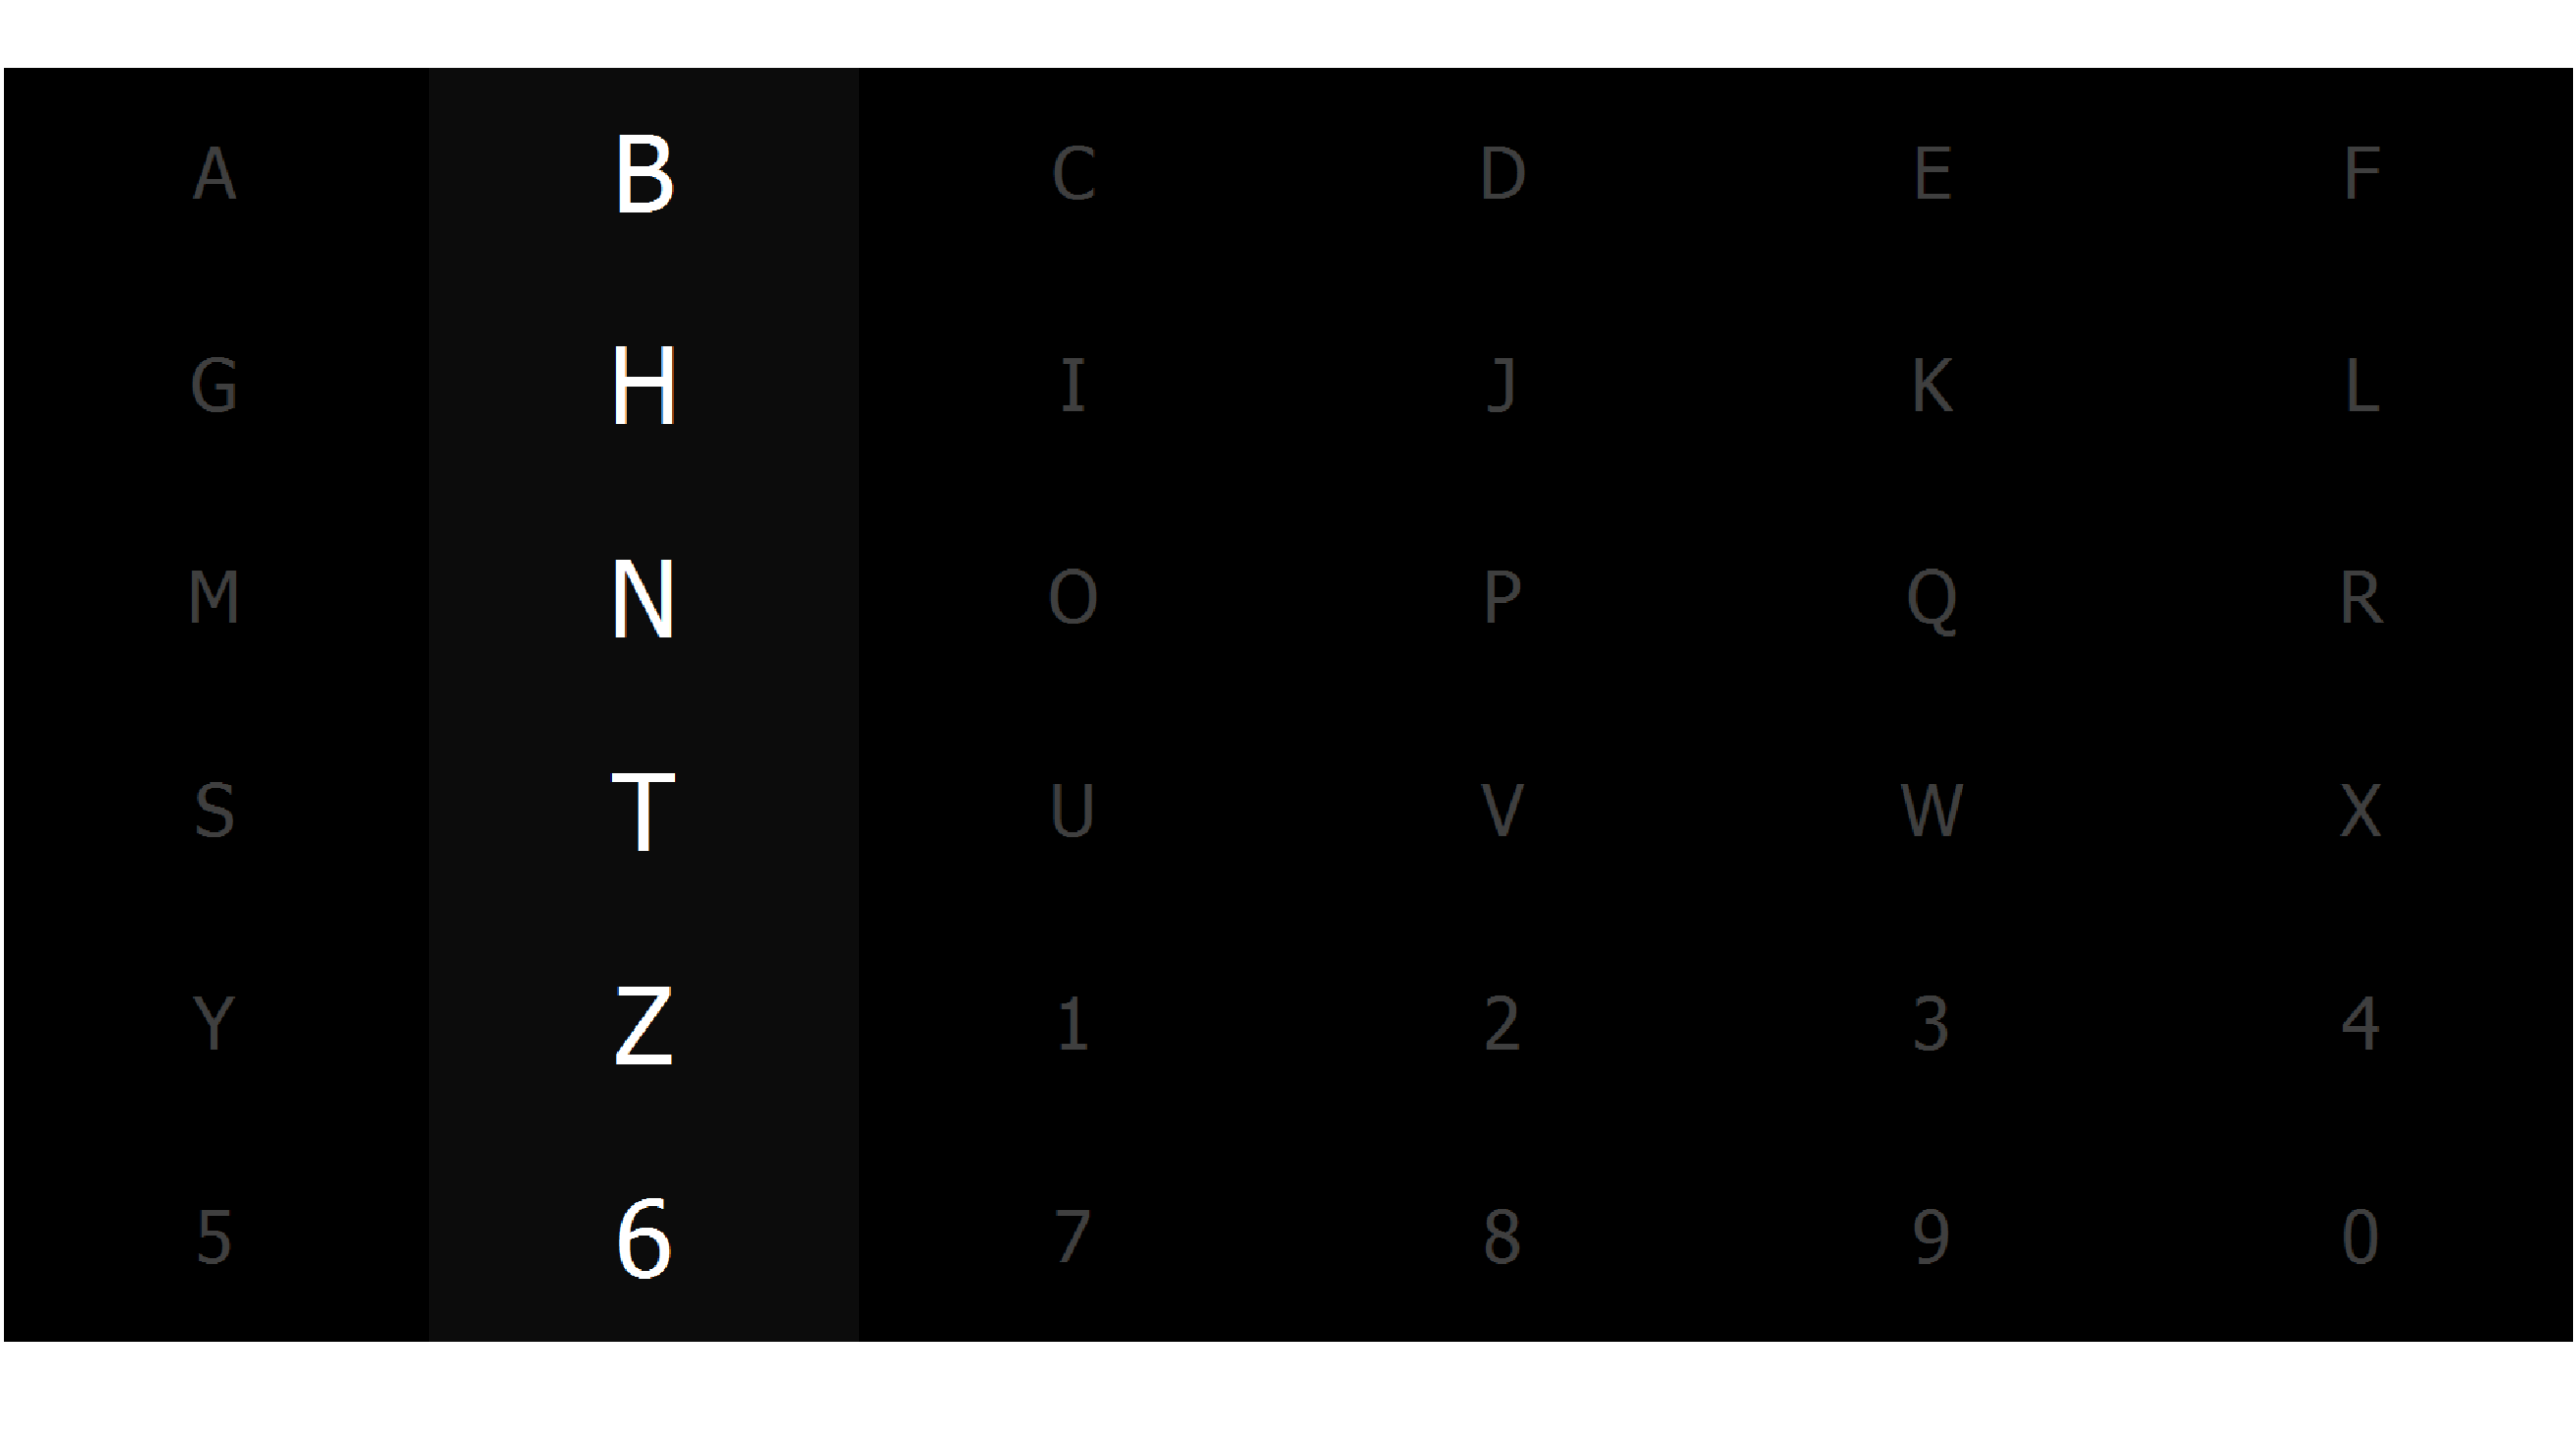
\includegraphics[width=0.5\columnwidth]{Figures/P300Speller.pdf}
    \caption{\footnotesize{A P300-speller screen} }
    \label{fig:P300speller}
\end{figure*}

%Performances were improved by adjusting the size of the stimulation matrix and the duration of the inter-stimulus interval [ref: Sellers 2006], by using the SSVEP evoked by the periodicity of the row/column flashing in the matrix to reinforce the detection of the target symbol.   
A considerable amount of work has been devoted to improving the machine learning algorithms for better detection of P300 \citep{hoffmann_boosting_2005,rakotomamonjy_ensemble_2005,zhang_p300_2007,krusienski_toward_2008,rivet_xdawn_2009,verschore_dynamic_2012,lenhardt_adaptive_2008,panicker_adaptation_2010}.
They have significantly contributed to the development of P300-based BCI.

Other stimulation paradigms, different from the row-column flashing matrix have been proposed, and yield good performances: for example using \emph{chequerboard paradigm} where individual characters are flashed randomly. 
In the chequerboard paradigm flashing objects or human faces improves ERP-based BCI \citep{hoffmann_efficient_2008,kaufmann_flashing_2011,kaufmann_face_2013,chen_survey_2015}. 
%[ref: Hoffmann-2008, ref: Kaufmann-2011-flash, Kaufmann-2013-face, Zhang 2014, Chen-2015-a-survey].

As stated earlier, the detection of P300 is done through averaging of repeated trials. This slows down the communication rate of the BCI.
An important trend in P300 BCI is the detection of P300 in a single trial. This is being achieved by experimental paradigms and signal processing technique that enhance the evoked P300 in a single trial and with adequate machine learning algorithms \citep{bayliss_single_1998,yin_novel_2013,ishita_development_2007,gucluturk_online_2010,kaufmann_comparison_2013} 
%[ref: Bayliss-1998-single, Yin-2013-a-novel-hybrid, Ishita-2007-dev, Güçlütürk-2010-an-online, Kaufmann-2016-comp]. 

Most of P300 BCI systems are synchronous; the timing is dictated by the stimulation system. 
Few implementations of asynchronous P300 BCI have been made. 
It is an effort to discriminate between control state (\textit{i.e.} P300 being elicited) and rest state (\textit{i.e.} the subject does not aim at any target), and to dynamically determine the number of trials needed for P300 detection \citep{lenhardt_adaptive_2008, zhang_asynchronous_2008, schettini_self-calibration_2014}.%, aloise_asynchronous_????} 
%[ref: Aloise-2010-asynch, Schettini-2014-self, Lenhardt-2008-an-adaptive, Zhang-2008-async]. 

Visual P300 stimulation presented thus far requires a gaze control from the subject, which is not achievable by locked-in patients.
A new paradigm was therefore developed to allow the use of visual P300 BCI by locked-in patient. 
%Individual or group of 
One or several characters are presented in a rapid sequence in the middle of a screen. 
In the stream of character, when the intended character is displayed (or magnified), a P300 should be elicited \citep{acqualagna_novel_2010, treder_gaze-independent_2011, aloise_covert_2012,  acqualagna_gaze-independent_2013}. 
%[ref: Acqualagna-2010, Acqualagna-2012, Treder-2011, Aloise-2012-a-covert]. 
Tactile P300 has also been investigated for locked-in patients \citep{kaufmann_comparison_2013}  

\subsubsection{Challenges in P300-based BCI systems}
\label{p300-challenges}

Amongst the limitations in P300-based BCI is the low information transfer rate, due to the repetition of trials required to enhance P300 extraction. 
Acceptable classification is obtained after more than 5 repetitions. 
In \citep{rakotomamonjy_ensemble_2005} for instance 15 repetitions are used and make a trial duration (\textit{i.e.} character epoch) of 35.4 seconds. 
This makes P300-based BCIs very slow. 
Single-trial detection approaches are a solution to this problem, but are hardly achievable. 

\par
The amplitude of the P300 decreases with time. 
The first occurrences of the rare stimuli will elicit a larger P300 \citep{courchesne_stimulus_1975} than the later occurrences will. 
This decrease might be explained by the local versus global probability of the rare stimulus. 
While the local probability of the rare stimuli within an oddball paradigm trial is the same over the entire BCI experiment, their global probability increases, creating a sense of habituation.
In a P300 speller paradigm, this is first observed at the character epoch level as the user gets used to the stimuli that are being repeated, and then over the sessions as the user becomes used to the nature of the rare stimulus. 
The amplitude of P300 will decrease with the habituation, thus deteriorating the BCI performance. 
A potential solution would be to consider the inter-trial variability of the P300 while training the classifier \citep{rakotomamonjy_ensemble_2005}.

\par
On the subject's side, although P300-based BCI systems do not require initial training, they require continuous attention from the user, who should pay close attention to stimuli and notice every time the rare stimulus occurs. 
Over the long run, this might be tiring for some subjects or just not achievable for those with attention disorders \citep{szuromi_p300_2010, krusienski_toward_2008}. 
%All else being equal, improving the methods used in the signal processing component will alleviate the challenges.

\subsubsection{Error-Related Potential}

The neural processing of incorrect response generate a negative going deflection (Ne) in the ERP.
The Ne has been observed in experiences with multiple-choice selection with tasks. Once a person observes an erroneous response, the error-related potential is elicited \citep{gehring_neural_1993}.

The error-related potential could thus improve the performance of non invasive BCI.
The erroneous action can either be automatically corrected or simply undone, as proposed by \cite{margaux_objective_2012}. The erroneous command is automatically replaced by the second most probable output of a probabilistic classifier.  
    
\label{errp}
\goodbreak
%##################################################################################################################################
\subsection{Visual Evoked Potential}
\label{subsec:vep}

%\subsubsection{Steady-State Visually Evoked Potential}

A Visual Evoked Potential (VEP) is an electrophysiological potential in the primary visual cortex in response to a visual stimulus. 
In general, a VEP contains three components illustrated in figure~\ref{fig:VEP}: a negative deflation at around 75 ms from the stimulus referred to as N75, a positive deflation at 100 ms from the stimulus referred to as P100, and a second negative deflation 135 ms after the stimulus called N135.

\begin{figure*}[!ht]
    \centering
    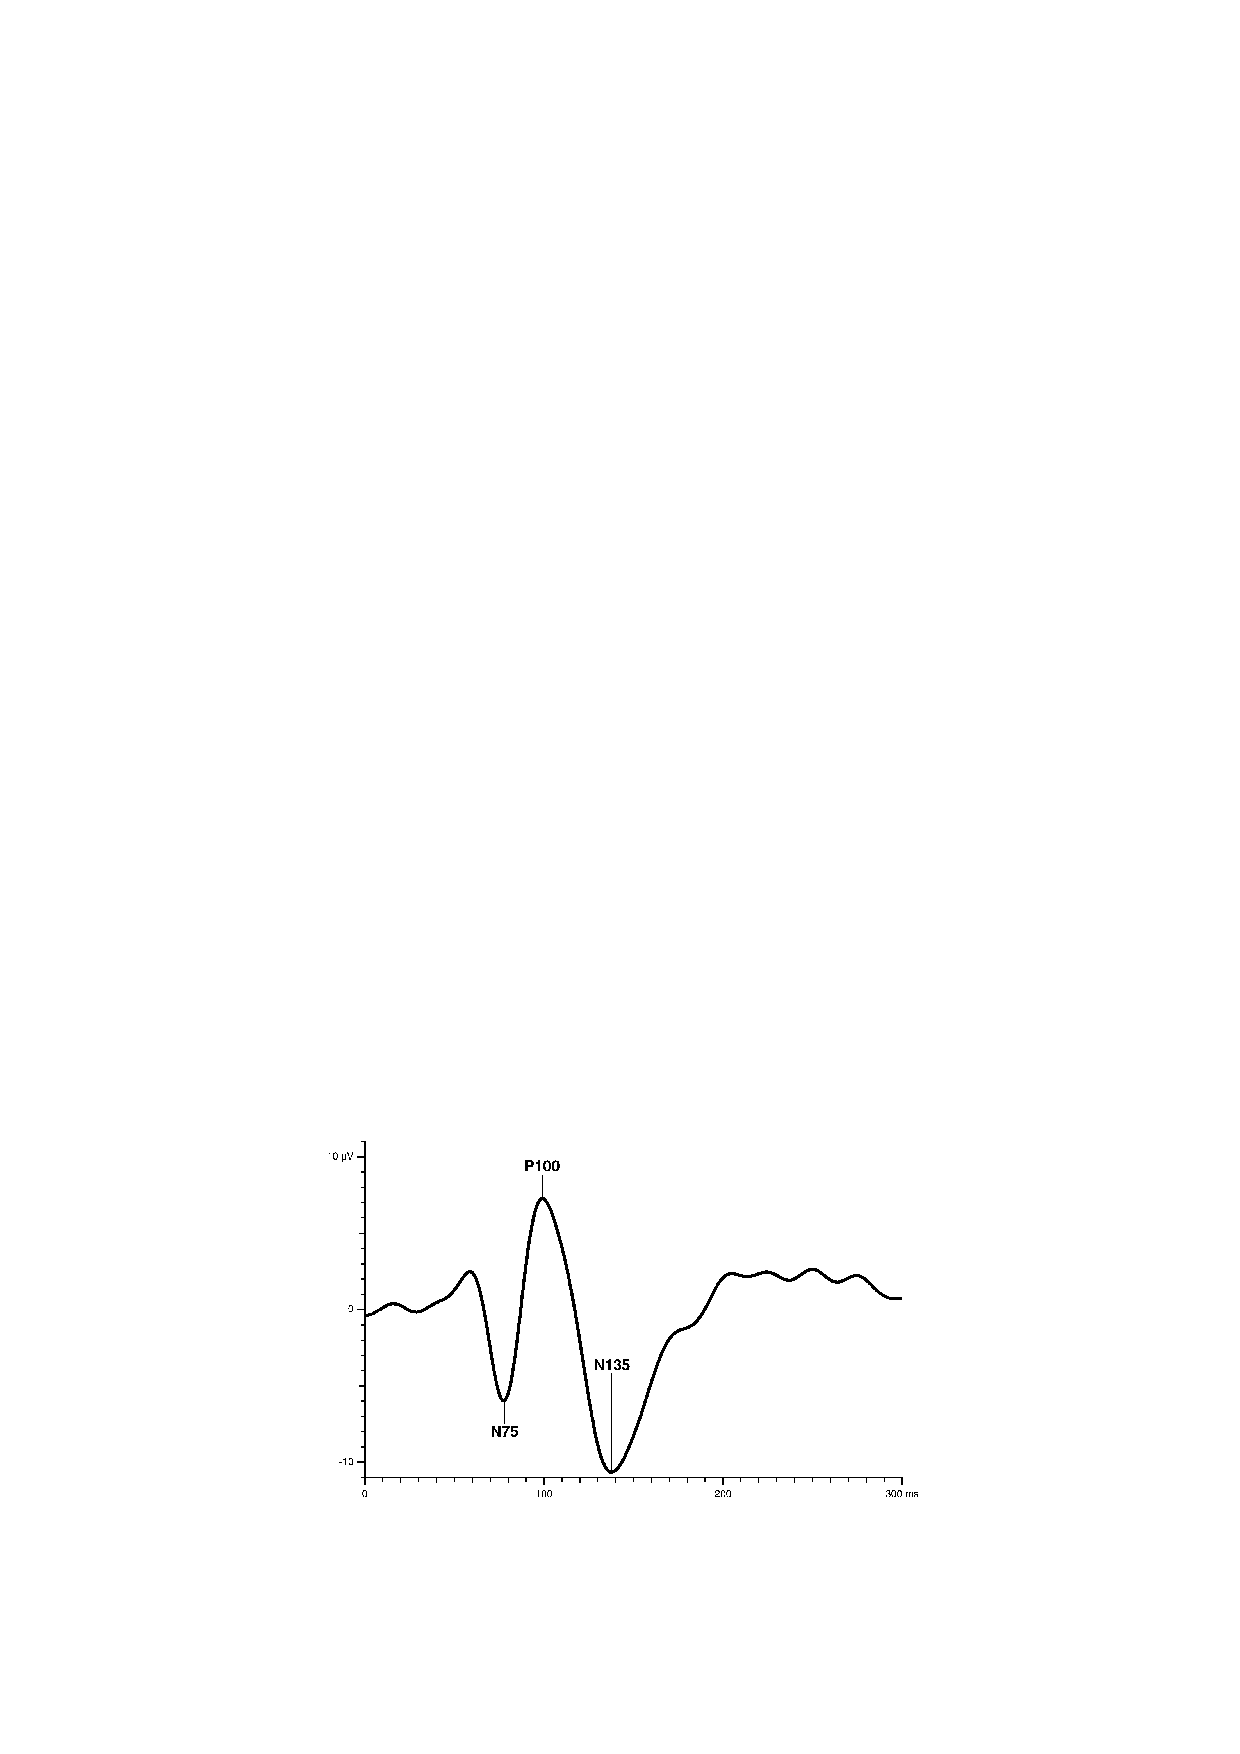
\includegraphics[width=0.5\columnwidth]{Figures/VEP.pdf}
    \caption{\footnotesize{A Standard Visual Evoked Potential} }
    \label{fig:VEP}
\end{figure*}
\par

VEP can be either transient or steady, \textit{i.e.} \emph{Steady-State Visually Evoked Potential} (SSVEP). 
Transient VEP can be defined as the response to an isolated or infrequent stimulus that provides enough time for the system to return to its initial state before onset of the next stimulus.
The steady state response of SSVEP corresponds to a periodic succession of transient evoked potentials \citep{capilla_steady-state_2011}. 
Neuronal activity in the primary visual cortex is synchronised at the stimulation's fundamental frequency and its harmonics. 
This phenomenon is being increasingly used in brain-computer interfaces.  

\begin{figure*}[!ht]
    \centering
    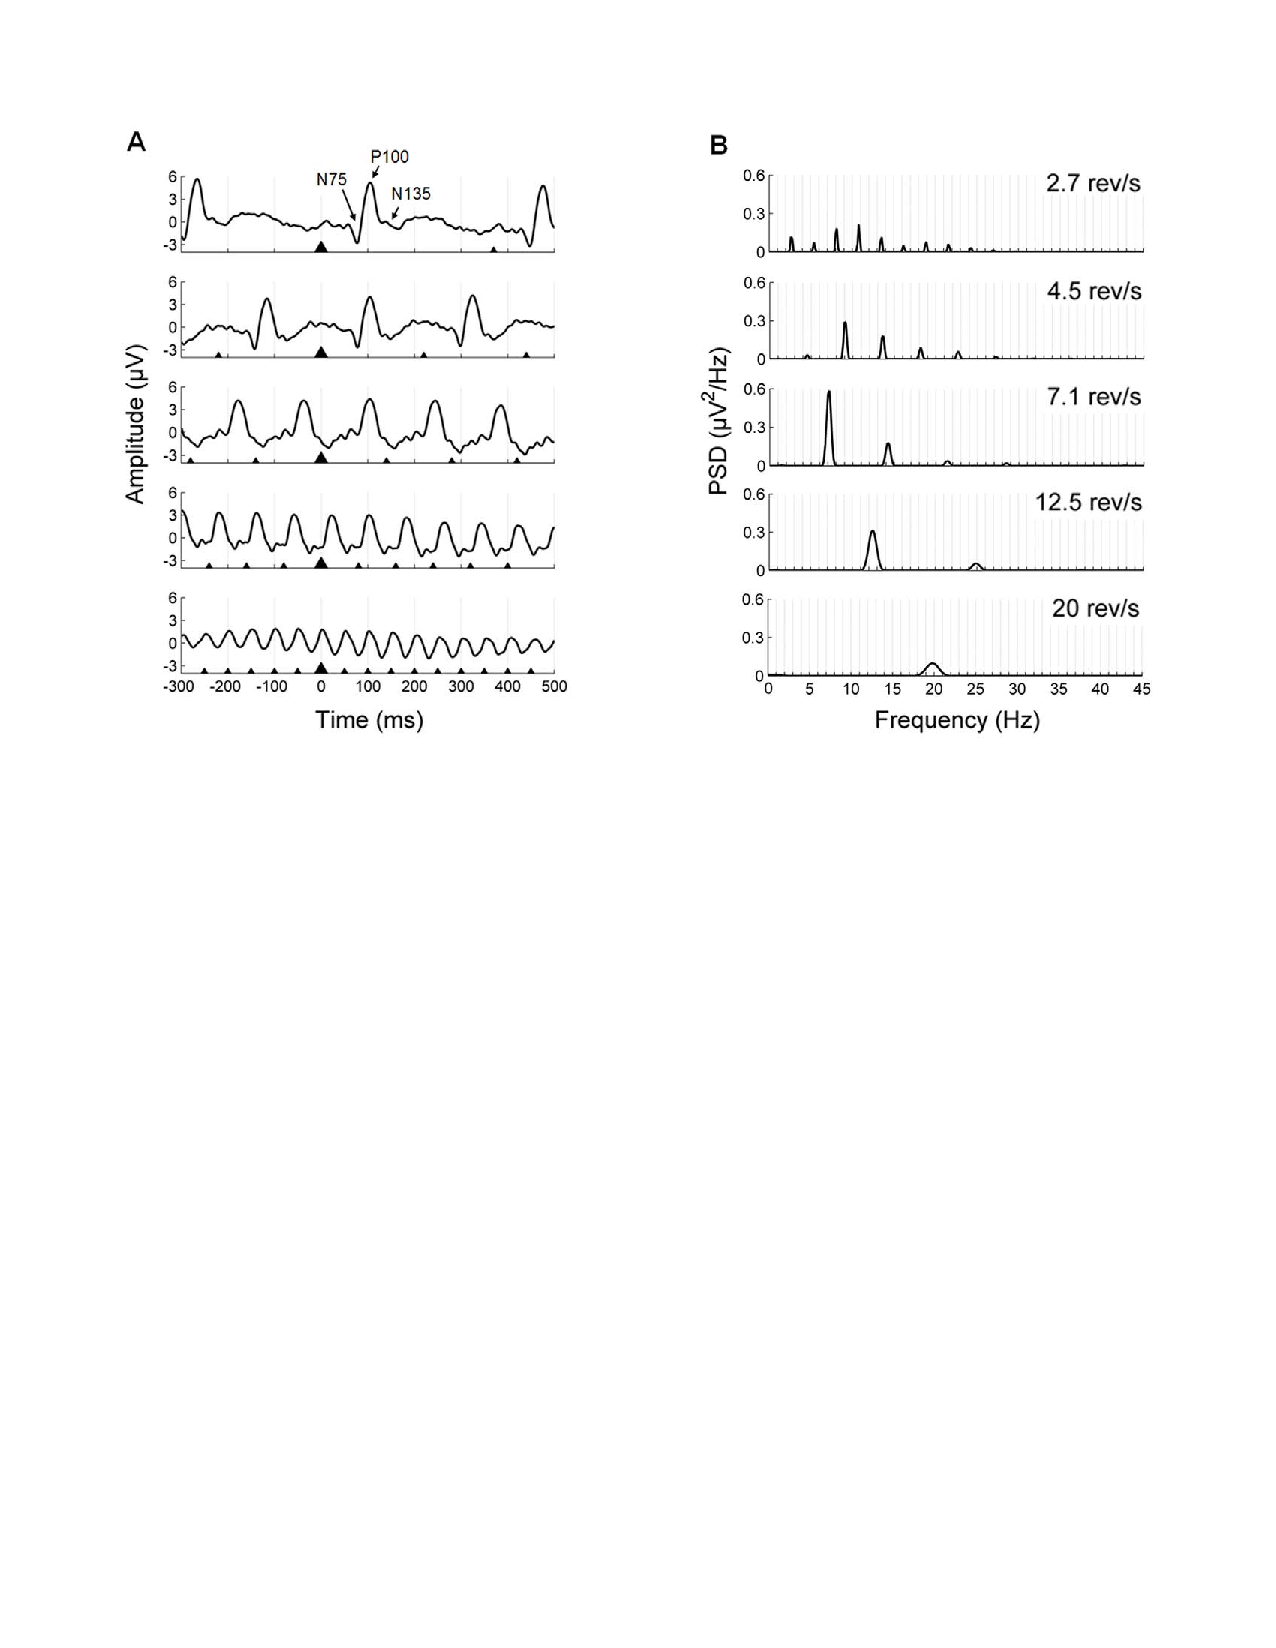
\includegraphics[width=0.5\columnwidth]{Figures/VEP-SSVEP.pdf}
    \caption{\footnotesize{Visual evoked potentials at stimulation frequency of 2.7 Hz, 4.5
            Hz, 7.1 Hz, 12.5 Hz, and 20 Hz. A illustrates the signal in time
            domain and B illustrates the frequency spectrum. \citep[Reproduced from][]{capilla_steady-state_2011} }. }
    \label{fig:VEP-SSVEP}
\end{figure*}
\par

Figure \ref{fig:VEP-SSVEP} is very expressive with regards to the nature of SSVEP. 
While all three major voltage deflation (\textit{i.e.} N75, P100, and N135 ) are observable in steady state responses at lower frequencies (e.g. 2.7 and 4.5 Hz) -- making them very similar to transient evoked responses, they are less visible when the frequency of the stimuli train is increased. 
Only the P100 is still present at all stimulation frequencies. The amplitude of the steady state response appears to be attenuating as the stimulation frequency increases. 
%Based on the conclusion that SSRs are a linear summation of transient responses, 
This attenuation can be explained by latent inhibition, meaning that the transient excitation of the neural generators responding to the first stimulus in a sequence spreads to neurons that, in turn, feed back to them, attenuating the response to an incoming stimulus.
High stimulation frequencies, with periods far shorter than the width of a P100, will suffer more from this inhibition.

\begin{figure*}[!ht]
    \centering
    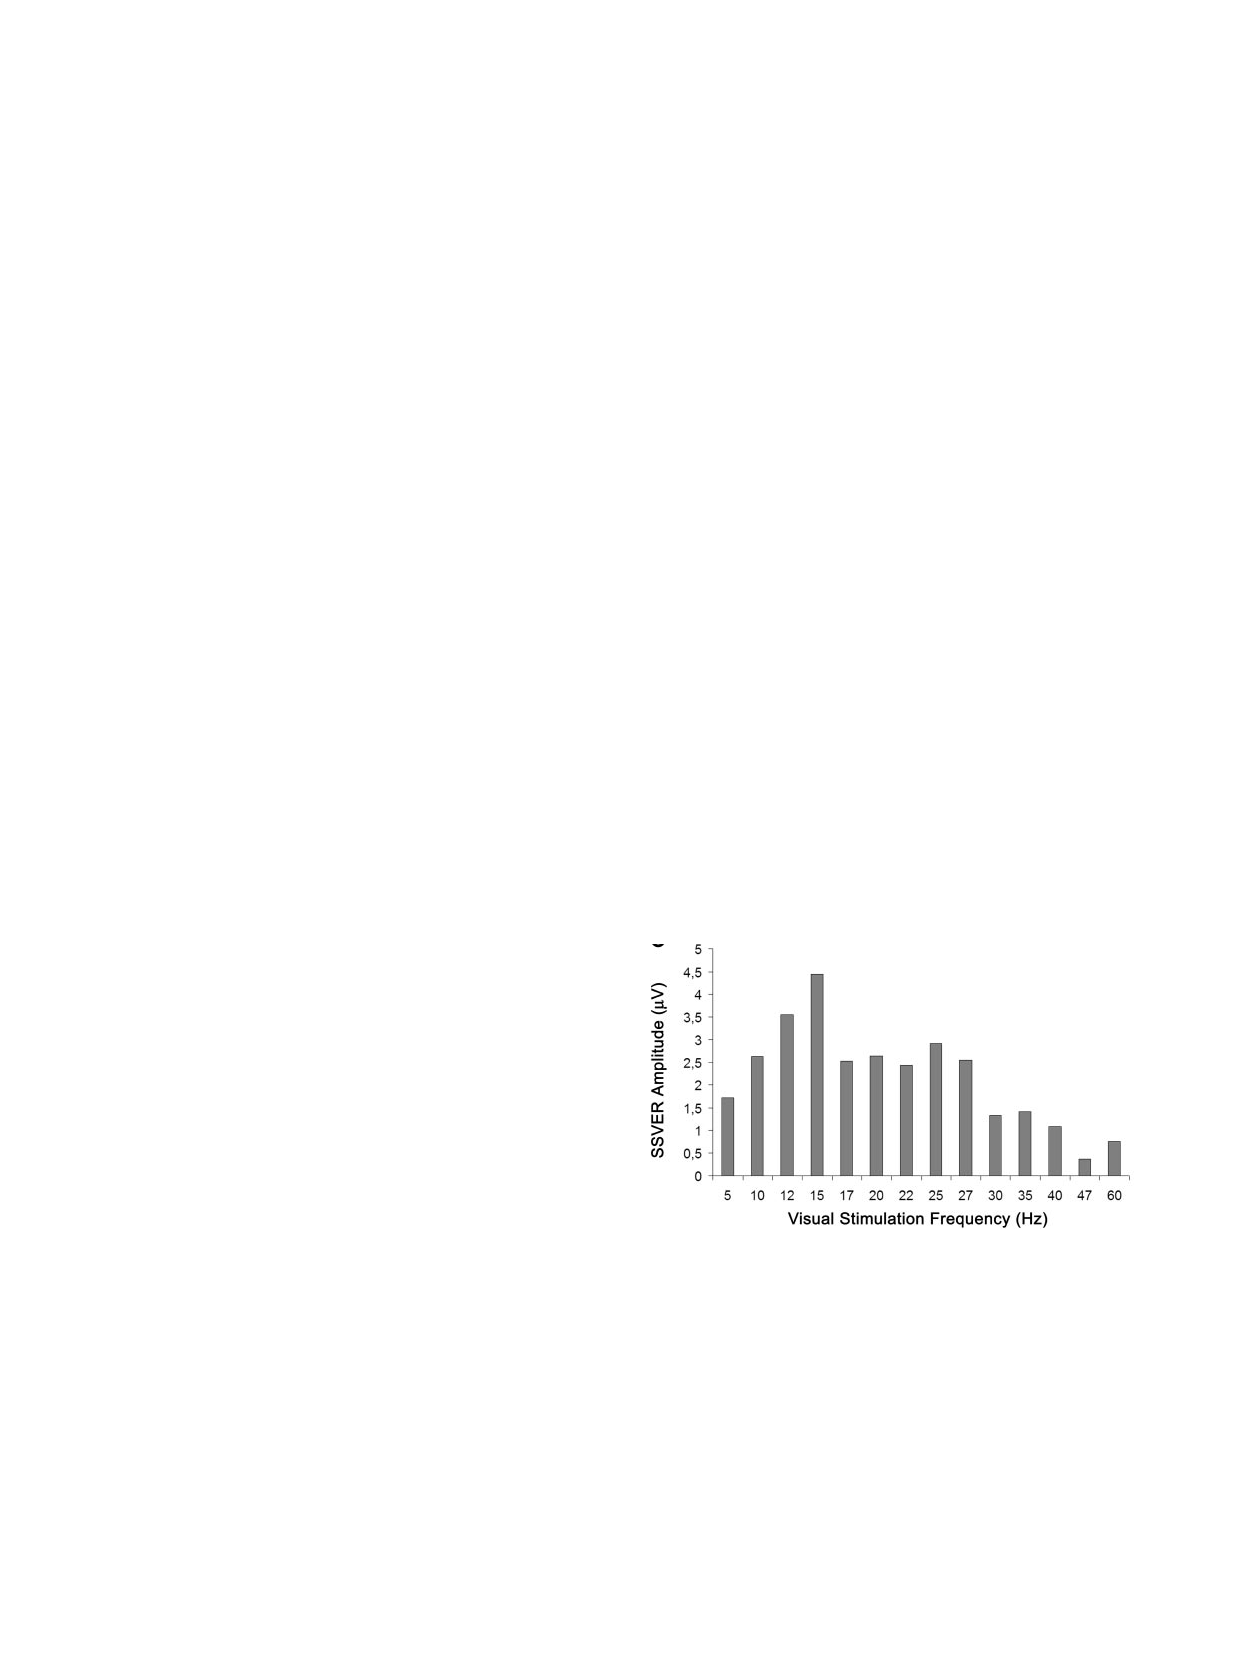
\includegraphics[width=4.0in]{Figures/SSVEP-frequencies.pdf}
    \caption{\footnotesize{Average of the
    mean values of the amplitude of the FFT fundamental frequency of the SSVEP
    recorded at the three occipital leads (Oz, O1, O2) at
    the different stimulation frequencies. The amplitude of the occipital SSVEP,
    expressed in microvolts, reached a maximum at 15 Hz and then fell, with a
    plateau up to 27 Hz, declining at higher frequencies. \citep[Reproduced from][]{pastor_human_2003}.}}
    \label{fig:SSVEP-frequencies}
\end{figure*}
\par

At lower frequencies ( $\le$ 7 Hz), the frequency component corresponding to the stimulation frequency is very weak. 
From 7 Hz up, this component is predominant. 
In both cases, harmonics of the stimuli frequency are visible especially for intermediate frequencies. 
The presence of harmonics is explained by the number of positive and negative voltage deflation found in a single VEP. 
At higher stimulation frequencies, the late deflation of preceding VEP cancel out (or overlap with) the early deflations of the ongoing VEP, leaving out a single VEP component per VEP. 
This explains the absence of harmonics in SSVEP from higher stimulation frequencies. 
With regards to amplitude of response, \cite{pastor_human_2003} reached similar conclusions in their studies. 
They show that responses to low and high stimulation frequencies are less visible than responses to intermediate frequencies (see Figure~\ref{fig:SSVEP-frequencies}). 
Another factor affecting the attenuation of responses to high simulation frequencies is the low pass filtering characteristics of the skull \citep{nunez_electric_2005, bedard_model_2006}.

\subsubsection{SSVEP-based BCI systems}

There are various techniques to design stimulus for SSVEP in BCI. They are reported in \citep{zhu_survey_2010}. 
Different simulation frequencies are used to build multiple BCI commands.
%Two categories of SSVEP stimulation techniques are used in BCI: Pattern stimulus and flash stimulus.
%Pattern stimulus can be divided into two: pattern reversal and pattern onset/offset.
%In pattern reversal stimulation, white and black checks are repeatedly reversing their colours at a specific frequency on a checkboard displayed on a screen. 
%A single reversal perceived by the subject elicits a VEP, while a train of reversals results in SSVEP. 
%For pattern onset/offset a pattern is abruptly exchanged with a diffuse background.
%Pattern reversals are easy to control and offer a noticeable contrast. 
%Flash stimuli on the other side are based on flashing lights. 
%Such stimuli are generated using either light emitting diodes (LED) or screens (\textit{i.e.} LCD orCRT). 
%The amplitude of the evoked potential strongly depends on the nature of the stimulus: its shape, size, color, intensity, contrast with the
%background, etc. 
%This is discussed in more detail in \cite{Zhu2010aSurvey}. %try citep[This is discussed in more detail in]{[ref:}
\par
As in other BCI systems, offline applications of SSVEP-based BCI are used to investigate the parameters influencing the performance of the system. 
SSVEP-based BCI, especially synchronous systems, have the advantage of focusing on EEG activity that occurs at known frequencies. 
Making use of this feature, many studies have reduced the feature extraction methods to a simple frequency spectrum quantification, e.g. Fourier transforms-based methods. 
The target whose stimulation frequency has the largest amplitude in the frequency spectrum of the brain signal recorded in the occipital region is considered to be the one that the
subject is gazing at \citep{muller-putz_control_2008, pfurtscheller_self-paced_2010}. 
Due to inter-trial and inter-subject variability of the frequency spectrum features, parameters optimisation methods are introduced or classifiers such as \emph{support vector machines} that can be trained and used to classify the frequency spectrum features into classes \citep{kalunga_ssvep_2013}.
Methods using canonical correlation analysis are very successful in the identification target's stimulus frequency \citep{lin_frequency_2006, kalunga_ssvep_2013, nakanishi_high-speed_2014}.
\par
Over the past years, interest in SSVEP-based BCI has increased due to the advantages it presents over other BCI systems. 
SSVEP have a higher signal-to-noise ratio, leading to higher classification accuracy, and a fast information transfer rate \citep{nakanishi_high-speed_2014}. 
Moreover, due to the fact that SSVEP is an inherent response of the brain, SSVEP-BCIs' users do not need to go through intensive training.
\par
It should be mentioned that the highest performances have been achieved in synchronous systems. 
Even in some asynchronous systems, the subjects are supposed to be continuously gazing at one target stimulus. 
This keeps the classification simpler as it avoids the complexity of discriminating between intentional control (IC) state and no-control (NC) state.
To alleviate the complexity of having to discriminate continuously between NC and IC, some BCI systems activate the SSVEP target stimuli only when needed.
Once the stimuli are activated, the system is invariably in the IC state, and when deactivated, it is in NC state \citep{cheng_design_2002, pfurtscheller_self-paced_2010}.

SSVEP-based BCI is often employed as a dependent BCI \citep{wolpaw_brain-computer_2000}, that is, some residual muscular capabilities are required to move the eye toward the blinking stimulus as opposed to independent BCI, such as Motor Imagery (MI), where the communication does not rely on any motor capability.
It has been shown that SSVEP could be used as an independent BCI \citep{morgan_selective_1996, muller_feature-selective_2006-1} as the brain oscillations are strongly related to the focus of attention.
Using covert attention, \textit{i.e.} shifting the focus of attention without moving the eyes, subjects can generate different SSVEP responses.%The subjects generate different SSVEP responses without moving their eyes, simply shifting their attention from one stimuli to another.

Visual stimulus plays a crucial role, affecting the BCI performance, and should be designed carefully.
An in-depth review of the literature shows that LED stimuli provide better results than those obtained on computer screen \citep{zhu_survey_2010, oralhan_effect_2016}.
A cognitive study indicates that any stimulation between 2 and 50 Hz induces visible oscillations in the visual cortex \citep{herrmann_human_2001}.
Common values employed in SSVEP studies are between 12 and 25 Hz, as they induce oscillations with higher amplitudes \citep{zhu_survey_2010}. 
One should note that safety of the subject should be taken into account as some frequency ranges of the stimulation could trigger epileptic seizure \citep{fisher_photic-_2005}. 

The phase of the stimulation signal can also be modulated, enhancing the BCI performance by boosting the Information Transfer Rate (ITR) \citep{pan_enhancing_2011, nakanishi_high-speed_2014}. % and a peak bitrate of 124 bit/min~\cite{VOL11}.
An important constraint in that case is that experimental setup requires a synchronization between the display and the recording system, to ensure the correct estimation of the stimulus' phase.
Better alternatives are available when considering systems with such constraints: code-modulated VEP (c-VEP) has yield the highest ITR in BCI \citep{spuler_one_2012, bin_high-speed_2011}.
In c-VEP, the sole difference is that the stimulus flickering is based on pseudorandom sequences instead of the fixed frequencies of SSVEP.

%All these successful approaches in SSVEP and c-VEP rely on CCA.
%Given two sets of signals, CCA aims at finding the projection space that maximises their cross-covariance while jointly minimizing their covariance \cite{Lin2007,kalunga2013ssvep,nakanishi2014high}.
%The common methodology is to find the canonical space between the multichannel EEG trial on the one hand and reference signals, usually sine and cosine of target frequencies and harmonics, on the other hand. 


\subsubsection{Challenges in SSVEP-Based BCI Systems}

Although SSVEP relies on the perception of the subject rather than eye movement, the majority of current SSVEP-based BCI paradigms requires eye movements for the perception of stimuli. 
To operate such systems, the subject must possess a functional visual system which should, moreover, entirely be devoted to the BCI application. 
Nonetheless, studies are investigating the possibility of an SSVEP-based BCI without the need of gazing \citep{lopez-gordo_high_2010}.
\par
%Another challenge is found in the limited number of usable frequencies for SSVEP stimuli.
%While increasing the number of targets in a SSVEP-based BCI is advantageous for the information transfer rate, the number of usable target stimuli is limited. 
This limitation is due to the fact that SSVEP can only be elicited within a limited frequency band. 
Also, due to the fact that harmonics of a stimulation frequency cannot be used in other target stimuli. 
Applications using computer monitors are faced with another limitation in usable frequencies due to the monitors refresh rates. 
The refresh rate must be a multiple of the stimulation frequency to avoid discrepancies in the generated frequency. 
\cite{jia_frequency_2011} proposed a stimuli coding method that combines frequency and phases. 
On a single frequency many stimuli can be coded using different phases, thus increasing the number of targets.
c-VEP is an alternative to SSVEP that does not have this constraint \citep{spuler_one_2012}.
\par
The implementation of asynchronous systems that can discriminate between IC and NC with minimal false positive still poses a challenge. 
This is crucial for real life applications, yet studies investigating the matter and evaluating the performance of such systems are very few in number when
compared to the attention SSVEP-based BCI have drawn in recent years.

\goodbreak
%##################################################################################################################################

\subsection{Discussion}
\label{subsec:neur_pheno_discussion}

The presented neurological phenomena have all been used with considerable success in BCI. 
They each have advantages and drawbacks.
The choice of a neurological phenomenon will depend on the specific needs in the BCI application.
An adequate threshold should be found between the efficiency of the system and the comfort of the BCI user.
Indeed the neurological phenomenon used in the BCI impact both the system's performance and the comfort of users.

In general, there is a duality or complementarity between endogenous and exogenous BCIs, the strengths found in one are usually the weaknesses found in the other.
While exogenous BCIs suffer from the fact that they depend on the muscular functions and on an external stimulus, endogenous BCI are free from this dependency; except visual P300 that might need gaze control.
Endogenous BCIs require that the user be trained, while exogenous BCI can be used with no training.
Endogenous BCI have very low signal amplitude, while their counterpart enjoy a relatively stronger signal amplitude.
Endogenous BCI are flexible; the user can shift between several mental tasks in a single BCI application. That is usually not possible with exogenous BCI.

%Endogenous 	-> pros=>Independent: Muscular system and exteranal stimulus (Exept vP300 that usually require ocular control)
%			-> cons=>Need training: P300 need lesser training 
%				   =>Poor signal amplitude
%Exogenous 	-> pros=>No need for training
%				   =>Good signal to noise amplitude
%			-> cons=>Dependence: Both on muscular and external stimulus

Hence, BCIs that rely on exogenous BCI cannot be used by patients in a complete locked-in state. 
With no muscular function left, they still retain sensory and cognitive abilities that can be leveraged in endogenous BCI.
There is however a vast population of patients who do retain gaze control, for whom visual techniques can still be used. 
Moreover, SSVEP and P300 are related to attention and perception rather than to gaze control. 
An appropriate BCI paradigm leverage this characteristic for their application in locked-in patients.
The dependence to perception and attention also marks the difference between evoked potential-based BCI (\textit{i.e.} P300 and SSVEP) and muscular devices such as eye-trackers, devices that rely on eye-fixation and saccades. 

BCI illiteracy can be observed with any type of BCI.
15 to 20\% of users cannot generate neurological responses necessary to control a particular BCI.
\cite{allison_could_2010-1} discussed the possible causes of illiteracy and proposed few potential solutions that mainly consist of improving BCI accuracy in general. 
An interesting observation is that a subject who is illiterate in one BCI modality (e.g. SSVEP) might effectively use another modality (e.g. ERD). 
Different neurological modalities could be combined in a hybrid interface, where their impact is weighted depending on the user's abilities. 
There are also questions being raised about changing current approaches to BCI altogether.
For example, recently \cite{jeunet_why_2016} challenged the standard training protocol used in MI-based BCI. 
They used the protocol followed in BCI tasks to train users on non-BCI task. They found that about the same rate 17\% of users could not perform the learnt task, which is about the rate of BCI illiteracy. 
Their findings suggest that the training protocol used in BCI is not optimal and might by a influential factor in BCI illiteracy.
These results will surely prompt more digging in approaches used in BCI.

%Une conclusion contenant les conclusin de toutes les section ?
%-------------------------------------------------------------------------